\documentclass[conference]{IEEEtran}

%     _      _____                    ____
%    / \    |__  /___ _ __ ___       |  _ \ ___ _ __   __ _ _ __ ___   ___
%   / _ \     / // _ \ '__/ _ \ _____| |_) / _ \ '_ \ / _` | '_ ` _ \ / _ \
%  / ___ \   / /|  __/ | | (_) |_____|  _ <  __/ | | | (_| | | | | | |  __/
% /_/   \_\ /____\___|_|  \___/      |_| \_\___|_| |_|\__,_|_| |_| |_|\___|
%
%   ____                          _ _   _
%  / ___|___  _ __ ___  _ __ ___ (_) |_| |_ ___ _ __
% | |   / _ \| '_ ` _ \| '_ ` _ \| | __| __/ _ \ '__|
% | |__| (_) | | | | | | | | | | | | |_| ||  __/ |
%  \____\___/|_| |_| |_|_| |_| |_|_|\__|\__\___|_|

%\usepackage{babel}
\usepackage{graphicx}
\usepackage{color}
\usepackage{cite}
%\usepackage{algorithmic}
%\usepackage{algorithmicx}
\usepackage[ruled,vlined,boxed]{algorithm2e}
\usepackage{listings}
%\usepackage{minted}
\usepackage{underscore}
\usepackage{multicol}
\usepackage{float}
\usepackage{checkend}
\usepackage{enumitem}

% ========================================================================
% commands


\newcommand{\SUCCESS}{\texttt{\_SUCCESS}\ }

% add a todo marker. We can turn this off when we don't want to see it.
\newcommand{\TODO}{\emph{TODO}\ }
\newcommand{\FOC}{\texttt{FileOutputCommitter}\ }


% ========================================================================


\title{
A Zero-Rename Committer:\\
Object-storage as a Destination\\ for Apache Hadoop and Spark}

% Yes, this titling is broken
\author{
  Loughran, Steve
  \texttt{stevel@apache.org}\\
\and
  Blue, Ryan
  \texttt{rblue@netflix.com}\\
\and
  Radia, Sanjay
  \texttt{sradia@apache.org}
\and
  Demoor, Thomas
  \texttt{thomas.demoor@wdc.com}
}

\date{December 2017}

% ========================================================================

\begin{document}


\maketitle

% ========================================================================

\begin{abstract}

We introduce new \emph{committers} for Apache Hadoop, which
the Amazon S3 Object Store to be safely used as a direct destination of output generated
by Hadoop MapReduce and Apache Spark.

By using the operations directly exported by the store,
most critically the multipart-upload mechanism, tasks within a distributed
query can upload their output to the final destination,
yet not materialize this data until the overall job is committed.
As a result, the committers meet the core requirement of the Hadoop and Spark commit
protocols: the output of the job is complete and consistent: it contains
all the output of the successful ``committed'' work, and none of the output of
tasks which were committed.
That this mechanism permits highly-performant commit operations is an added benefit.

We also document the commit protocols of Hadoop and Spark, and show how the classic committer
implementation's requirements of atomic file creation and rename operations mean that they
cannot be safely used with Amazon S3.

We introduce our the two committers, ``Staging'' and ``Magic'', exploring their differences.
The Staging committer stages all generated output to the local filesystem of
worker nodes, uploading this data when a task is committed.
The Magic committer streams data directly to the object store, relying on the
object store client to recognise some output paths as special (``magic''), and
so translating writes to these paths as initiating a delayed-completion write
to a calculated final destination.

\end{abstract}

% ========================================================================

\section{Introduction}
\label{sec:introduction}

It has long been a core requirement of ``Big Data'' computation platforms that
the source and destination of data was a fully consistent distributed filesystem.

Distributed, because data needs to be readable and writable by the distributed
processes executing a single query across the cluster of computers.
Consistent, because all machines across the cluster need to be able to
list and read data written by any of the others.
As for ``Filesystem'', that's the model and API for distributed storage which
developers are familiar with.


The full semantics of a POSIX filesystem are not always necessary;
random write access to a file being an oft-omitted feature of the stores,
forcing the persistence formats to rely purely on appending data.

What has been a critical part of the required semantics has been that the filesystem
presents a model of directories and files with consistent operations to list and
read those directories and their contents, with at least four atomic operations:

\begin{itemize}
  \item Rename of a single file to another location within the same volume.
  \item Rename of a directory and its contents to another location within the same volume.
  \item Create a file iff a file or directory does not exist at that part.
  \item Recursive delete of a directory.
\end{itemize}

These operations are regularly used by applications as the foundational operators of higher-level
co-ordination and commit protocols.

For example, the \texttt{create()} operation can be used to obtain a lock on a resource:
the first process to create a file can consider itself having exclusive access to it,
and so implicitly consider itself to have acquired the resource.

The \texttt{rename()} operation is generally critical to providing atomic promotion
of output: a single \texttt{rename()} call can promote all in-progress output
of a worker to become completed work, simply by moving all the output to a well known path.
And, when the job completes, its final output may be renamed to a new location to become
publicly visible.

As covered in the original MapReduce paper\ \cite{MapReduce}:

\begin{quote}
We rely on the atomic rename operation provided by the underlying file system
to guarantee that the final file system state contains just the data produced
by one execution of the reduce task.
\end{quote}


Apache Hadoop was written with its own filesystem, Hadoop Distributed File System
(HDFS)\ \cite{Chansler2011}.

It is self-admittedly sub-POSIX as data can only be
appended directly to the end of the current file.
What it does offer is the classic filesystem model of
a tree of directories and files,
and the atomic operations needed by MapReduce to safely use HDFS
as a destination of work.
As will be shown, some object stores do not provide the same guarantees,
and so cannot be safely used as a destination with the standard protocol,
even if everything \emph{appears} to work.


% ========================================================================

\section{The Hadoop MapReduce Commit Protocol}
\label{sec:hadoop-mr-commit}

Before the challenge and solution of using an object store as a destination
of work can be covered, the problem of outputting data from a distributed
query itself must be covered, along with the existing protocols and algorithms.


\subsubsection{Terminology}

First, some terminology needs to be introduced to describe
the protocols.


\textbf{Query}.
One or more transformations of source data to a result;
data presented or saved in some form.
The query may be described in procedural source code,
or declaratively in a form such as SQL\@.


\textbf{Job}.
A parallelized query, composed of one or more distributed \emph{tasks}.
The output of a Job is made visible to other stages in a larger operation
sequence or other applications iff the job \emph{completes successfully}.
A complex query may consist of a chain of Jobs, either executing in sequence
or as a DAG of jobs.

\textbf{Job Attempt}.
A single attempt at executing a job.

\textbf{Task}.
Part of a job, such as a single Map or Reduce transformation applied to a fraction
of the input data.


\textbf{Task Attempt}.
A single attempt to complete a task on a single process running on a single host
in the cluster.
A task attempt is \emph{successful} if it generates all its output without
failing in some way.
A task attempt has \emph{failed} if the execution raises an exception, or
if the process executing the task attempt stops communicating with
the process managing the job.

Multiple attempts may be made to execute a task;
sequentially, if addressing task failure, or in parallel when task attempts are
executed speculatively.
It is critical that only one task attempt's output is propagated
to the final output of a job.


\textbf{Job Manager}.
The application which schedules task attempt execution, tracks success/failures,
determines when a job has been completed and publishes the results.
It may also determine that a job has failed and cannot be recovered,
in which case the job is aborted.

\textbf{Executor}.
A process capable of executing work, as directed by the Job Manager.
In Hadoop MapReduce, a unique executor is created for each partition
of the data, destroyed when the processing is completed.
In Spark, executors are long lived and can be allocated task attempts from multiple
jobs to execute, often simultaneously.

\textbf{Job Output Directory}.
The directory into which the output of a job writing to the filesystem is placed
so as to be visible.
After a successful job completion, the data MUST be visible in the destination
directory.

\textbf{Task Working Directory}.
A directory for exclusive access by a single task attempt, into which uncommitted
work may be placed.
All data written in and under this directory is considered the output of
that task attempt.


\textbf{Task Commit}.
The act of taking the output of a task attempt
and promoting it to become part of the final output of the active job
attempt.
When the output is a filesystem, this consists of moving the files
under the Task Working Directory and moving to the Job Output Directory,
preserving the hierarchy of subdirectories.


\textbf{Job Commit}.
The act of taking the output of all committed tasks of a job attempt,
and generating the final output.
This normally consists of publishing this output in an aggregate form;
it can also include generating extra summary data.
As this it is often a serialized operation at the end of a job attempt,
its performance can be a bottleneck.

\textbf{Task Abort}.
To cancel a task such that its data is not committed.

\textbf{Job Abort}.
To cancel all work in a job attempt: no task's work is committed.


\textbf{Job Context}.
An instance of the Java class \texttt{org.apache.hadoop.mapreduce.JobContext},
which provides a read-only view of the Job for the Job Driver and tasks.

\textbf{Task Attempt Context}.
An instance of the class
\texttt{org.apache.hadoop.mapreduce.TaskAttemptContext},
which provides operations for tasks, such as getting and setting status,
progress and counter values.


\subsection{Requirements of a Commitment Protocol}
\label{subsec:commit-protocol-requirements}

Apache Hadoop's MapReduce implementation is designed to support long-lived
large-scale queries taking minutes to hours to complete.
Its requirements include the following:

\begin{enumerate}

  \item Support for thousands to tens of thousands of individually scheduled $tasks$
  within a single $job$.

  \item Support different destinations of work, such as databases and
  distributed filesystems.

  \item ``Correctly'' propagate the output of individual tasks to the final
  aggregate of the job.
  What constitutes correctness is covered in\ \ref{sec:correctness}.

  \item Recover from the failure of a task attempt by rescheduling the task;
  a new task attempt may be executed anywhere within the cluster.

  \item Support speculative execution of task attempts as a means of compensating for the
  delay caused by \emph{stragglers} in the execution.

  \item Potentially: recover from a failure of a job attempt, using all the committed
  task output from the previous, failed attempt.

  \item Be resilient to network failures/partitions of tasks, and of the job manager
  itself becoming isolated from other parts of the system (and hence: a second
  attempt at the job being started).

\end{enumerate}

This leads to some specific requirements of an implementation, requirements
which can be used to assess its correctness.

\textbf{Independent.}
Individual tasks must be able to output without directly
co-ordinating that write with those of other tasks.

\textbf{Speculative tasks until committed.}
Multiple tasks must be able to simultaneously execute on the same input
source, to generate the required output of that part of the input.
This is required for recovery, and for speculation.
Non requirement: idempotent output;
that is left to the implementors of the operations executed in the tasks.

\textbf{Scaleable communication protocol.}
The commit protocol communications between task and job manager
must be support tens of thousands of simultaneous tasks.

\textbf{Abortable.}
It must be possible to abort an uncommitted task or job.
There should be no leftover output.

\textbf{Recoverable or Restartable Job.}
A committer can declare whether or not it supports job recovery;
if it does, it must implement recovery.
If not, the job must be restartable from the beginning.

\begin{figure*}
  \centering
  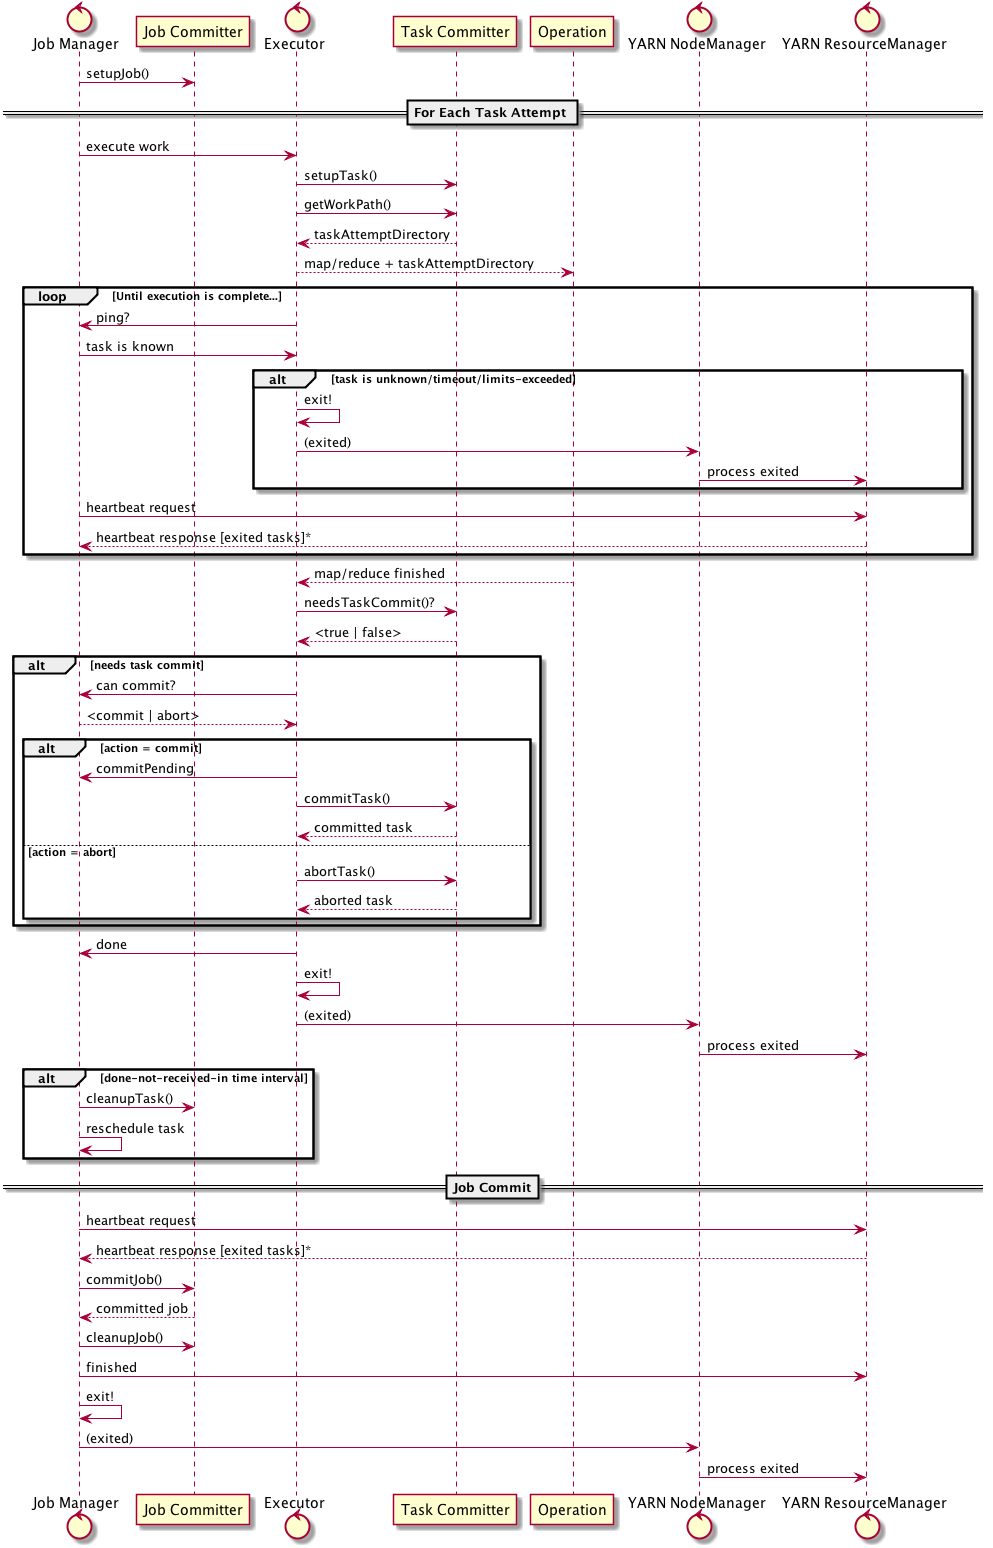
\includegraphics[width=.8\textwidth]{commit-protocol.png}
  \caption{Hadoop commit protocol (excluding Job recovery)}
  \label{fig:commit-protocol}
\end{figure*}

An UML sequence diagram of the core commit protocol is
show in\ \ref{fig:commit-protocol}.

The commit algorithm is designed to work on the YARN cluster scheduler
\ \cite{Vavilapalli2013}.

On each node in the YARN cluster, a \emph{Node Manager} has the responsibility
of launching the applications, usually within a memory-and-CPU-bounded
environment.
A central \emph{Resource Manager} manages the scheduling liveness monitoring
of individual applications.
When an application is submitted for execution, the Resource Manager schedules
its root process, the \emph{Application Master}.
This communicates with the Resource Manager via an umbilical protocol
which is explicitly used by the application for requesting new processes
across the cluster, and implicitly used by the Resource Manager
as a liveness probe of the application.

When a launched process terminates, the process exit code
is passed to the \emph{ResourceManager} within the regular status heartbeats
between each NodeManager and the ResourceManager.
If it is the Application Master itself which has terminated, unless it explicitly
declared itself to be finished, the application is considered to have failed.
All worker processes will be terminated (by default), and a new instance
of the Application Master scheduled for execution.
If it was a worker process, the Application Master chooses how to    react.


In MapReduce, the YARN Application Master is the Job Manager,
with every individual task attempt executed in a unique worker process, termed
an ```executor'' in this paper.
A direct RPC protocol between the Job Manager and the executors is used to manage
the commit operation.
Excluding process failures, all liveness detection must be performed by the
Job Manager, which is done based on timeouts of this direct RPC protocol.

% -----------------------------------------------------------------------

\subsection{Recoverable Failure Modes}
\label{subsec:optionalRecoverableFailureModes}

\subsubsection{Job Recovery}

When YARN perceives the Job Manager process to have failed, it instantiates
a new instance of the process somewhere within the cluster.
This new Job Manager creates an instance of the specified Job Committer,
and queries it as to whether job recovery is supported.

If a committer does support recovery.,
the state of the previous job attempt is rebuilt from reading the
``Job History'' file.
This file is a log of the events saved during the execution, including
a record of all tasks which successfully committed, and which could
therefore be recovered.
The Job Committer's \texttt{recoverTask(TaskAttempt)} method is called
for each of these tasks.
All unexecuted, uncommitted or unrecoverable tasks are scheduled for execution.

If job recovery is not support the entire job is re-executed.

As the probability of the Job Manager failing is, excluding bugs in the code itself,
a function of job time, rather than scale, recovering from job failure is more
important on long lived jobs ---those which last many hours.

\subsubsection{Bad Records}

To avoid an entire task, and hence job, failing due to a single unprocesseable record,
task attempts may skip records whose processing raises an exception.
If the number of skipped records in a task attempt is below some threshold
threshold, these records will not result in a task attempt reporting itself as
having failed.
This is not of direct relevance to the commit protocol except as a
reason for a task attempt to fail.

\section{Hadoop's FileOutputCommitter}
\label{sec:fileoutputcommitter}



The operations to commit the work, the Task Commit and the Job Commit,
are all implemented in the same class, an implementation of \texttt{OutputCommitter}.
For writing to HDFS, this is done in the \texttt{FileOutputCommitter} class.

This actually implements two separate algorithms for committing work: each
with different performance and scalability characteristics.

The ``v1'' algorithm was designed to handle failure and recovery with an
atomic task commit and the ability to explicitly recover the output generated
by the committed tasks of a failed job attempt.

The ``v2'' algorithm was added in 2015, as its predecessor was found
to have scalablity problems for jobs with tens of thousands of files
\ \cite{MAPREDUCE-4815}.
While the v2 algorithm can deliver better performance, it comes at the price of
reduced isolation of output.

\textbf{v1.}
When a task attempt is committed, its task working directory is renamed into
the job attempt directory.
When the job attempt is committed, all committed task directories are merged
(serially) into the job output directory.
A restarted job move the directories of committed tasks from the previous
attempt, so recovering their output.


\textbf{v2.}

When a task attempt is committed, its output is immediately merged into the
job output directory;
the job commit operation does nothing but create a marker file.
This is faster, but intermediate work is visible.
The task commit operation is no longer atomic, changing failure modes.

%\begin{table}
%  \caption{Attributes of the \texttt{FileOutputCommitter} algorithms}
%  \begin{tabular}{ l c c }
%    \hline
%    & \textbf{v1} & \textbf{v2} \\
%    Independent & True & True \\
%    Speculative Tasks & True & True \\
%    Recoverable Job & True & False \\
%    Abortable Job & True & Delete output directory \\
%    Observable & False & True \\
%    Atomic Task Commit & True & False \\
%    Idempotent Task Commit & True & False \\
%    Atomic Job Commit & False & True \\
%    Idempotent Job Commit & False & True \\
%    \hline
%  \end{tabular}
%  \label{tab:file-committer-attributes}
%\end{table}

\subsection{Common Variables}
\label{subsec:common-variables}


\begin{table}
  \caption{Variables used in the algorithms}
  \begin{tabular}{ l l l }
    \hline
    \textbf{name} & \textbf{meaning} \\
    $fs$ & Destination filesystem \\
    $destPath$ & Job Output Directory in the destination filesystem. \\
    $jobId$ & Numeric Job ID $\geq$ 0; expected to be unique for all application instances in the cluster. \\
    $jobAttemptId$ & $JobID_\$counter$; Counter starts at 0 for a job and increments on each attempt.\\
    $jobAttemptPath$ & a path under which a job attempt may store any data.\\
    $partId$ & Numeric value of partition of data to be allocated to a task.\\
    $taskId$ & $jobAttemptId_\$partId$; the task which works on part $partId$ in the job attempt.\\
    $taskAttemptId$ & $taskId\$counter$; a single attempt to execute a task.\\
    $taskAttemptPath$ & a path under $jobAttemptPath$ into which a task attempt may write uncommitted data.\\
    $taskCommittedPath$ & a path under $jobAttemptPath$ where the contents of $taskAttemptPath$ are moved when that attempt is committed. \\
    \hline
  \end{tabular}
\label{tab:variables}
\end{table}

For a Job Attempt $jobAttemptId$ to be successful, all parts of the dataset
must be processed in one or more successful tasks.
The output of exactly one task attempt for each task must be in the final dataset,

The function of a commit algorithm, then, is to guarantee that this condition
is met, even in the presence of failures.
It is not a requirement for an algorithm to be able to recover from all
failures;
it may react to some failure conditions by failing the entire job.

It is also not a general requirement that if a job fails, the job output directory
must be unchanged.
Together, this implies that at-most-once semantics are required,
and that the task of handling job failures is to be handled
by a higher-level workflow.

\subsection{Hadoop V1 commit algorithm}
\label{subsec:hadoop-v1-commit-algorithm}

%% Define the standard commit variables
\newcommand{\FileOutputCommitVars}{
\DontPrintSemicolon
\SetKwData{fs}{$fs$}
\SetKwData{dest}{$destPath$}
\SetKwData{jobAttemptPath}{$jobAttemptPath$}
\SetKwData{jobAttemptId}{$jobAttemptId$}
\SetKwData{SUCCESS}{_$SUCCESS$}
\SetKwData{taskAttemptId}{$taskAttemptId$}
\SetKwData{taskAttemptPath}{$taskAttemptPath$}
\SetKwData{taskCommittedPath}{$taskCommittedPath$}
\SetKwData{temp}{_$temporary$}}

\newcommand{\true}{ $true$ }
\newcommand{\false}{ $false$ }


\textbf{Job Setup}

This creates the path \emph{jobAttemptPath}, under the
directory \texttt{\_temporary} of the output directory
\emph{destPath}.

\begin{procedure}
\FileOutputCommitVars
% Operations, which are defined for all subsequent procedures/functions
% ALL functions must go in here, in alphabetical order
% Macros cannot have numbers in them, though their values can.
\SetKwFunction{abortUpload}{abortUpload}
\SetKwFunction{checkForConflicts}{checkForConflicts}
\SetKwFunction{commitJob}{commitJob}
\SetKwFunction{completeUpload}{completeUpload}
\SetKwFunction{delete}{delete}
\SetKwFunction{exists}{exists}
\SetKwFunction{Exception}{Exception}
\SetKwFunction{getFileStatus}{getFileStatus}
\SetKwFunction{getJobAttemptPath}{getJobAttemptPath}
\SetKwFunction{getUsername}{getUsername}
\SetKwFunction{isDirectory}{isDirectory}
\SetKwFunction{isFile}{isFile}
\SetKwFunction{listFiles}{listFiles}
\SetKwFunction{listPendingUploads}{listPendingUploads}
\SetKwFunction{loadPendingFile}{loadPendingFile}
\SetKwFunction{loadPendingSet}{loadPendingSet}
\SetKwFunction{mergePathsA}{mergePathsV1}
\SetKwFunction{mergePathsB}{mergePathsV2}
\SetKwFunction{mkdir}{mkdir}
\SetKwFunction{mkdirs}{mkdirs}
\SetKwFunction{newUUID}{newUUID}
\SetKwFunction{rename}{rename}
\SetKwFunction{return}{return}
\SetKwFunction{savePendingSet}{savePendingSet}
\SetKwFunction{tempDirForStaging}{tempDirForStaging}
\SetKwFunction{throw}{throw}
\SetKwFunction{touch}{touch}
\SetKwFunction{uniquePath}{uniquePath}
\SetKwFunction{uploadFileToPendingCommit}{uploadFileToPendingCommit}

  \jobAttemptPath $\longleftarrow$ \dest/\temp/\jobAttemptId\;
  \mkdir(\fs, \jobAttemptPath)\;

\caption{setupJob()}
\label{alg:FileOutputCommitter.setupJob}
\end{procedure}

Note Hadoop has a convention that all paths starting with ``_'' are not considered
``visible'';
everything under this directory is excluded from normal
listings of the destination path.
Creating all intermediate files in a subdirectory of the destination
directory provides an implicit guarantee that the data is created in the
same volume (in a multi-volume filesystem), and in the same encryption zone,
for any HDFS cluster with encryption enabled.


\textbf{Task Setup}

The task attempt is given a directory under the job attempt path
as its task working directory.

\begin{procedure}
\FileOutputCommitVars

  \taskAttemptPath $\longleftarrow$ \jobAttemptPath/\taskAttemptId\;

\caption{setupTask()}
\label{alg:FileOutputCommitter.setupTask}
\end{procedure}

The actual directories are created on demand.


\textbf{Needs Task Commit}

A commit is required iff data was generated.

\begin{function}
\FileOutputCommitVars

  \exists(\fs, \taskAttemptPath)\;

\caption{needsTaskCommit()}
\label{alg:FileOutputCommitter.needsTaskCommit}
\end{function}

This is somewhere where any eventual consistency of object listings in an object
store can generate a false ``no data to commit'' negative result.

\textbf{Task Commit}

A task attempt is committed simply by renaming the task attempt working directory
into the job attempt directory.

\begin{procedure}
\FileOutputCommitVars

  \If{\exists(\fs, \taskAttemptPath)} {
    \delete(\fs, \taskCommittedPath, $recursive$)\;
    \rename(\fs, \taskAttemptPath, \taskCommittedPath)\;
  }

\caption{commitTask()}
\label{alg:FileOutputCommitter.commitTask}
\end{procedure}


In a true file system, the rename is an $O(1)$ atomic operation.
%Even if the task fails to report to the Job Manager that the
%commit operation was completed, the existence of the \texttt{taskCommittedPath}
%is an implicit confirmation that the task was committed.
%Its absence is not a guarantee that the task has failed ---it could just
%be taking slow to execute the operation.
%However, the Job Manager can assume that the task has failed,
%and reschedule another attempt at that task.
%Whichever of the rescheduled or original (delayed/partitioned) task
%last renames their task attempt path to the task committed path is considered
%the successful committer.

\textbf{Task Abort}

Abort a task attempt by deleting its task attempt path.

\begin{procedure}
\FileOutputCommitVars

  \delete(\fs, \taskAttemptPath, $recursive$)\;

\caption{abortTask()}
\label{alg:FileOutputCommitter.abortTask}
\end{procedure}


On a genuine filesystem this is an $O(1)$` operation.
%On an object store, usually $O(files)$.

\textbf{Job Commit}

A Job is committed by merging all files/directories in from all the task
committed paths into final job output directory.

Optionally, it can create a zero-byte `\SUCCESS` file in the output directory.

\begin{procedure*}
\FileOutputCommitVars

  \For { committedTask $\in$ listFiles(\fs, \jobAttemptPath) } {
    \mergePathsA(\fs, committedTask, \dest)\;
  }
  \touch(\fs, \dest/\SUCCESS)\;
  \delete(\fs, \temp)\;

\caption{commitJob()}
\label{alg:FileOutputCommitter.commitJob}
\end{procedure*}


The \texttt{mergePathsV1(FileSystem, Path, Path)} procedure is
a recursive move of all the output of a committed task into/underneath.
the destination directory.

% ------------------------------------------------------------
\begin{procedure*}
\FileOutputCommitVars

  \eIf { \isFile(\fs, $src$) } {
    \If { \exists(\fs, $dest$) } {
      \delete(\fs, $dest$, $recursive$)\;
    }
    \rename(\fs, $src$, $dest$)\;
  } {
    \eIf { \exists(\fs, $dest$) } {
      \eIf { \isFile(\fs, $dest$) } {
        \delete(\fs, $dest$, recursive)\;
        \rename(\fs, $src$, $dest$)\;
      } {
        \For { f $\in$ \listFiles(\fs, $src$) } {
         \mergePathsA(\fs, f, $dest$ + f.name)\;
        }
      }
    } {
      \rename(\fs, $src$, $dest$)\;
    }
  }

\caption{mergePathsV1(fs, src, dest)}
\label{alg:mergePathsV1}
\end{procedure*}
% ------------------------------------------------------------

All the files and directories are promoted to the destination directory.

\begin{enumerate}
  \item If the calculated destination path of a source file or directory does
  not exist, the source files/directory renamed.
  \item If the destination path does exist and is a file, it is deleted and then
  the source files/directory renamed.
  \item If the destination path exists and is a directory, and the source
  is also a directory, then \texttt{mergePathsV1} is applied to the child
  entries of the source path.
\end{enumerate}

Together, it forms a depth-first overwrite of the source tree by the destination
tree, specifically merging the contents all directories.

%This is clearly not an atomic operation;
%it is performing a sequence of operations on the distributed filesystem,
%potentially including recursive operations down a directory tree.
The time to execute the merge depends on the number of source entries
and the state of the destination directory.

If it fails, the state of the operation is unknown: it cannot simply
be repeated.


\begin{function}

  \false

\caption{v1.isCommitJobRepeatable()}
\label{v1.isCommitJobRepeatable}

\end{function}

Accordingly: if a job attempt fails during the commit process, it is
unrecoverable: the subsequent attempt reports an error and aborts.

% Abort Job v1
\begin{procedure}
\FileOutputCommitVars

  \delete(\fs, \jobAttemptPath, $recursive$)\;

\caption{v1.abortJob()}
\label{alg:v1.abortJob}

\end{procedure}

A job attempt an be cleaned up by deleting the output of all job attempts which
may have been made.
This can be achieved by deleting the entire \texttt{_temporary} directory
under the destination directory.

% cleanup job v1
\begin{procedure}
\FileOutputCommitVars

  \delete(\fs, \dest/\temp, $recursive$)\;

\caption{cleanupJob()}
\label{alg:v1.cleanupJob}
\end{procedure}

This would break with any other ongoing job which is writing to the
same destination directory.
It is a requirement that only one job may be actively writing
to a specific destination, something which is checked for during job submission.


\textbf{Job Recovery}

The v1 committer can recover from a failed job attempt, with the
second attempt being able to reuse the output of all committed tasks from
the previous attempt.

This job whole attempt recovery process is a complex one;
from the perspective of the committer, if the task attempt was committed
in the previous job attempt, the $taskCommittedPath$ of the previous attempt
can be moved under the $jobAttemptPath$ of the new job attempt.


\begin{procedure}
\FileOutputCommitVars

  \delete(\fs, \dest/\temp, $recursive$)\;

\caption{isRecoverySupported()}
\label{alg:v1.isRecoverySupported}
\end{procedure}


\begin{procedure}
\FileOutputCommitVars

  $previousJobId$ = $jobId$ - 1
  $previousJobAttemptDir$ = getJobAttemptPath($previousJobId$ - 1)
  \delete(\fs, \dest/\temp, $recursive$)\;

\caption{recoverTask(TaskAttemptContext )}
\label{alg:v1.recoverTask}
\end{procedure}


The only lost work is that of all in progress task attempts ---those which had generated
data but were not yet committed.

When working with HDFS, the main limitation of this algorithm is
one of scale: job commit is an $O(tasks)$, with the time for
each task's merge being a function of the number of files and the depth of
the directory tree.

As this is serialized at the end of the job, irrespective of how many workers
there were, the job commit is a single point of delay, and of failure.
The more tasks, the more work to commit, the longer the commit, and the
higher risk of that failure.

\subsection{Hadoop V2 commit algorithm}
\label{subsec:hadoop-v2-commit-algorithm}


The v2 commit algorithm propagates the task attempts output into the job's
output directory in the task commit.
This is done in a variant \texttt{mergePaths()} algorithm,\ \ref{alg:mergePathsV2},
designed to support parallel writers to the output directory.
In the Hadoop source the two algorithms are intermixed within a pair of
co-recursive procedures;
they have been isolated here for clarity.


% ------------------------------------------------------------
% V2 commit algorithm
\begin{procedure*}
\FileOutputCommitVars

  \eIf {\isFile(\fs, $src$)} {
    \If {\exists(\fs, $dest$)} {
      \delete(\fs, $dest$, $recursive$)\;
    }
    \rename(\fs, $src$, $dest$)\;
  } {
    \eIf {\exists(\fs, $dest$)} {
      \eIf {\isFile(\fs, $dest$)} {
        \delete(\fs, $dest$, $recursive$)\;
        \mkdirs(\fs, $dest$)\;
        \For {c $\in$ \listFiles(\fs, $src$)} {
          \mergePathsB(\fs, c, $dest$ + c.name)\;
        }
      } {
        \For {f $\in$ \listFiles(\fs, $src$)} {
          \mergePathsB(\fs, f, $dest$ + f.name)\;
        }
      }
    } {
      \mkdirs(\fs, $dest$)\;
      \For {f $\in$ \listFiles(\fs, $src$)} {
         \mergePathsB(\fs, f, $dest$ + f.name)\;
      }
    }
  }

\label{alg:mergePathsV2}
\caption{mergePathsV2(fs, rc, dest)}

\end{procedure*}
% ------------------------------------------------------------

Here, the \texttt{rename()} operation is restricted to committing
a single file: whenever a directory is to be committed, it is done
as a recursive merge.
This is necessary because multiple tasks may be committing simultaneously, tasks which
may be writing to the same destination.
The atomic exclusivity of a directory rename is precisely what is not
wanted when trying to support multiple tasks merging their output into the
same directory tree.

Performance-wise, the \texttt{mergePathsV2} operation is slower
than the v1 algorithm whenever there are directories to commit.
Yet, because these operations are taking place in task commits, work is parallelized
across the cluster, and, often, not directly slowing down the overall job.

With the file propagation taking place in the tasks, the job commit
operation is reduced to creating the \SUCCESS file and cleaning up
working directories:

\begin{procedure*}
\FileOutputCommitVars

  \touch(\fs, \dest/\SUCCESS)\;
  \delete(\fs, \temp)\;

\label{alg:commitJobV2}

\caption{v2 commitJob()}
\end{procedure*}

As a result, the time to commit a job is barely measurable.

In terms of failure resilience, the v2 algorithm is weaker than the v1 algorithm.
Task commit is now a non-atomic operation;
It is therefore not possible to safely recover from the failure or loss of a task attempt
while it was committing work.

Because the output of committed tasks are visible,
if the job fails the contents of all committed tasks are visible.

This commit algorithm has chosen speed over resilience.

This is often a valid decision to make, however, the callers of the committers
need to be aware that this decision has been made, and that failures in
certain parts of the process, specifically task commit, are not recoverable.

\subsection{Limitations of the Hadoop MapReduce Commit Protocol}
\label{subsec:hadoop-commit-protocol}

Alongside some implementation details, such as the fact that a task process
will be exit without calling \texttt{cleanupTask()} once it is informed that it
is unknown, we have to consider: are there any fundamental issues with
the Hadoop commit protocol?

A key weakness is that the job committer is not passed the list of task
attempts considered successful, and, from those committed tasks, their
lists of files which were committed.

The committers themselves have to implement some mechanism to determine this
of tasks.
The File Output Committer does this through the filesystem, relying on consistent
metadata listings to enumerate task output to merge, and, for the v1 algorithm,
to enumerate the set of committed tasks whose output must be published in job commit.
This places a requirement for the filesystem metadata listings to be consistent,
a requirement not met by all not object stores.

As no list of completed tasks is directly passed to the \texttt{commitJob} operation,
the job committer cannot determine whether the actual committed output
in the filesystem is correct.

There also appears to be a race condition between
verification that the destination directory does not exist in the
the client-side job submission, and the creation of that directory during
the \texttt{setupJob()} operation.
In a busy cluster there can be a delay between the scheduling of the job and
its application manager actually starting to execute\ldots
a second, conflicting, job may also be scheduled at this point.
If the destination directory were to be created during job submission,
this window would be nearly completely eliminated.

% ========================================================================

\section{The Spark Commit Protocol}
\label{sec:spark-commit-protocol}

Apache Spark's execution model is significantly different from
that of Hadoop.
Rather than dedicate a single process to executing a single operation
across a subset of the source data, Spark creates a set of \emph{Executors},
each of which can execute task attempts across a number of threads.
As a result, a single executor may be executing many task attempts
simultaneously, with each task's commit operations being centrally managed
by the single Job Manager.

\begin{figure*}
  \centering
  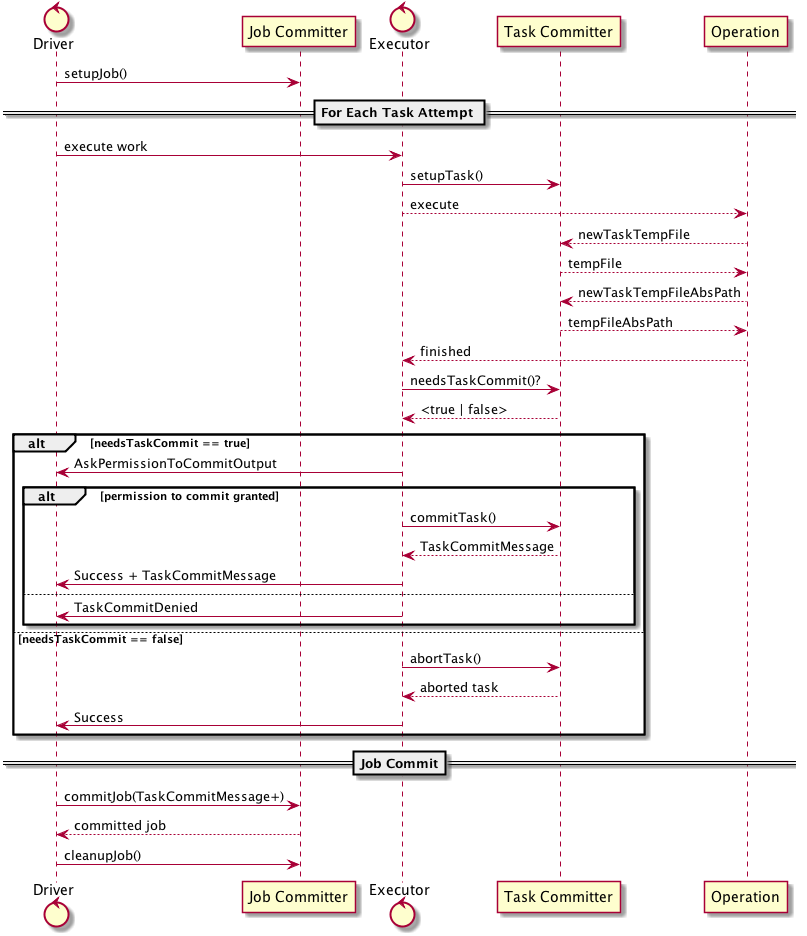
\includegraphics[width=.8\textwidth]{spark-protocol.png}
  \caption{Spark commit protocol)}
  \label{fig:spark-protocol}
\end{figure*}


When a failure of an executor is detected by loss of its heartbeat,
all active tasks will be rescheduled.
As the failure may be a network partition, multiple task attempts may be active
simultaneously.
It is therefore a requirement that no data is promoted until a task attempt is actually
committed.


Spark can use the Hadoop Committers within its commit protocol,
which is usually done whenever writing data to HDFS or other cluster filesystem.

Spark manages its requirement of ``only one task attempt may be committed''
in its \texttt{OutputCommitCoordinator} class;
an instance of this in the driver tracks the state of all active task attempts
and grants or denies permission to commit.

A task attempt is only granted permission to commit if a set of conditions
are met\footnote{see: \texttt{OutputCommitCoordinator.handleAskPermissionToCommit()}}:

\begin{enumerate}
  \item The task attempt is not recorded as having failed.
  \item The task attempt is in the set of known-to-be active tasks
  \item Either the requesting task attempt has already been granted this permission,
  no task attempt has been granted permission to commit, or a previous task
  was granted permission, but it is considered to have failed.

\end{enumerate}

That is: it must be a valid task attempt and no other task attempt can be
actively committing or have committed this task.

The Executor requests this permission to commit via an RPC call and will
proceed with the commit when it receives a successful message.
A timeout on the RPC channel or a denial of commit permission will result
in \texttt{abortTask()} being invoked.

Once a task attempt has been granted permission to commit, then no other
attempt will be granted unless the first attempt is reported as having failed.

\TODO: \texttt{OutputCommitCoordinator} reacts to task events from the scheduler, but
does that cover executor failure?

Spark makes no attempt to recover from a failed Job Manager;
its mechanism for recovering from a failed job is ``rerun the entire query''.

One area where Spark goes beyond Hadoop's protocol ias that
it adds a new operation to request a file with an absolute path,
 \texttt{newTaskTempFileAbsPath()}.
It is needed to address the special case of Apache Hive, wherein
some parts of the dataset are written to different locations than
under the destination directory of a job.
The operation, having calculated the absolute destination of the output,
requests a temporary file which will be placed in the final destination
directory on a job commit.

Spark implements this operation atop the standard \texttt{FileOutputCommitter}
as follows:

\begin{enumerate}
  \item An ``absolute path staging directory'' is created under the job output
  directory;
  this is \texttt{_temporary-\$jobId}.
  \item When a \texttt{newTaskTempFileAbsPath()} is invoked, a path under this
  directory is generated, with a UUID in the filename.
  \item The mapping of absolute path to temporary file is stored in a map in the Task Committer.
  \item In the \texttt{commitTask()} operation, the map of all files to rename is passed back.
  \item In \texttt{commitJob()}, after invoking the Hadoop committer's \texttt{commitJob()}
  call, all files in the aggregate map of files to rename to absolute paths is iterated through.
  Each file is renamed to its final path, in turn.
  \item Task abort will delete files of that task, while Job abort will delete
  the whole absolute path staging directory.
\end{enumerate}

This is extra operation is currently only used in that specific use case,
``Hive table with partitions elsewhere in the same filesystem as the active job''.
This is not a common use case, at least with data stored in object stores.
Accordingly, our new committers do not support this operation
\footnote{It is possible to support this, but it would complicate cleaning up
after tasks, especially failed ones, and failed jobs.}.

Spark is more flexible in its commit protocol, because
the name for a file is generated by the committer, not the application,
and because successful task committers can pass arbitrary serialized data back
to the driver, for use in the Job Commit operation.
This could potentially be used as the sole mechanism for passing a list
of written files from the task attempts to the job committer.
Being able to generate names (albeit while preserving a sort order), could
also be potentially useful.
We have initially chosen to not explore this as a commitment strategy;
others may wish to do so.



\subsubsection{Limitations of the Spark Commit Protocol}

The standard commit coordination in the Spark Driver is with the
\texttt{OutputCommitCoordinator}.
this class's state includes tracking whether or not a task attempt
has been granted permission to commit its work.
Once one task attempt has been granted permission to commit,
all other task attempts for the same task will be denied.
However, if the task attempt granted permission to commit its work fails
for any reason, the attempt is considered a failure, and
another attempt will be granted permission to commit its work.

This strategy works, provided task commit is a repeatable operation,
even if the first attempt has failed or become partitioned from the
Spark Driver.
That requirement is met for the \texttt{FileOutputCommitter} v1 algorithm,
but possibly not by the v2 algorithm, or, potentially, others.
If committers could declare their ability to recover from
failed task commits, along with other aspects of their operation,
the \texttt{OutputCommitCoordinator} would be able to decide whether
a repeated attempt were permitted, or whether failing the Job was the
safer outcome.


Unlike the Hadoop protocol, there is no requirement for the Spark Driver
to have received a recent liveness check from the cluster scheduler.
Unless the Spark Driver process exits once it determines that it has been
isolated from any underlying cluster scheduler, there is a risk that
a partitioned Spark cluster may commit a job to the same destination
as a cluster instantiated as a replacement.
Careful review of the YARN and Mesos integration code is required to be
confident that this risk does not exist.

Spark's commit protocol permit task committers to return data to
the Job Committer in the Spark Driver;
it would be possible to use this to validate the output of the tasks.
The current committer implementations do not do this, but at least the underlying
protocol makes such an improvement possible.




% ========================================================================

\section{The Challenge of Object Stores}
\label{sec:object-stores}

Having introduced the classic filesystem and the commit protocols and algorithms
used to commit the output of distributed computation, let us consider
Object Stores such as Amazon S3, Google Cloud Storage and
Windows Azure Storage\ \cite{AWS-S3-intro,Calder11}.

% As all filesystem
%operations are via the NameNode, all clients get a consistent view of the filesystem.
%And, as the


The most salient point, is this: Object Stores are not filesystems.
Rather than the classic hierarchical view of directories, subdirectories
and paths, object stores store a set of objects, each with a unique key;
a sequence of characters provided when the object was created.
Classic path separators ``\texttt{/}'' are invariably part of the set of valid
characters, so allowing objects to be created which have the appearance
of files in a directory.

As examples, the following are all valid keys on the Amazon, Google and Microsoft
stores

\begin{verbatim}
/entry
/path1/path2/path3
/path1/
/path1
\end{verbatim}

More subtly, it is valid for an object store container (on S3:, a ``bucket'')
to have objects with all of these names simultaneously.
It is not an error to have an object whose key would make it appear to be
``under'' another object, nor to explicitly contain path entries separators.

Objects cannot generally be appended to once created, or renamed.
They can be replaced by new objects or deleted.
Some form of copy operation permits an object to be duplicated, creating
a new object with a different key.
Such copy operations take place within the storage infrastructure with a
copy time measurable in megabytes/second.


The set of operations offered are normally an extended set of HTTP verbs:

\begin{description}[leftmargin=8em, style=nextline]
  \item[PUT] Atomic write of an object
  \item[GET] retrieve all or part of an object
  \item[HEAD] retrieve the object metadata
  \item[LIST] list all objects starting with a given prefix
  \item[COPY] copy a single object within the store, possibly from other containers.
  \item[DELETE] Delete an object
\end{description}

There are usually two extra operations to address scale:
 a bulk delete call which may have partial failures,
and \emph{Multipart Upload}; a way to upload an object larger than the
5GB which a single HTTP POST can support.
The exact nature of multipart uploads varies from store to store.
For Amazon this is initiated as a sequence of POST calls, one to initiate,
one or more POST calls with data, and a final POST listing the (ordered)
etags of the uploaded object parts.
All but the last upload in the object must be 5 MB or larger


Object store implementations can display different levels of inconsistency.
Windows Azure Storage is fully consistent;
Amazon S3 offers create consistency on new objects, but not updated or deleted ones.
It also exhibits listing inconsistency, wherein a newly created object
may not be visible in the results of a \texttt{LIST} call, or a newly deleted
object still be listed as present.


Despite the clear mismatch between the capabilities and APIs of object storage,
and that expected of a Hadoop filesystem, they have one key thing in common:
they can store Petabytes of data.
For that reason, all the popular cloud storage infrastructures have connectors
from Hadoop, and thus transitively application such as Apache Hive, Apache HBase
and Apache Spark.
Many of these are developed within the Apache Software Foundation's own
source repository, including the Azure ``wasb'' connector and the ``s3a'' connector
to Amazon S3.
Others are maintained externally ---particularly Amazon EMR's own ``EMRFS'',
known by the \texttt{s3} URL schema, and the Google Cloud Storage connector,
\texttt{gcs}.

Irrespective of where they are implemented, they all share a common objective:
trying to maintain the filesystem metaphor atop an object store.

As an example of a simple case, the \texttt{getFileStatus()} call mimics
a directory, in conjunction with zero-byte ``empty directory'' markers,
so must look for a file, then a marker and the most expensive operation, a path listing.

\begin{verbatim}
  GET path
  GET path/
  LIST path/
\end{verbatim}

The performance differences of every HTTPS request slows
down all RPC operations, even with pooled collections: even this simple probe
can for a file take hundreds of milliseconds.
Other mimicked operations have similar costs.

Operations upon directories are mimicked by listing all objects under that path,
and acting upon those objects individually.
A recursive delete is implemented as a listing of the maximum number of files
returned in one HTTP request (5000 or a similar value), then either issuing
bulk DELETE operations, where supported, or falling back to individual DELETE
calls.
Bulk LIST/DELETE operations have a cost of one HTTP request/page size, such
as $O(1 + descendants/5000)$; if sequential delete operations must be issued, then
the cost is at least $O(1+ descendants)$, with the ``at least'' qualifier being
added because request throttling can slow down the requests even further.

File and directory renaming is even more expensive.
A file rename is implemented as a copy of the original data to a new path,
followed by a delete of the original data.
This makes the time to copy single file an $O(length(file)$ operation.

Directory rename is a paged listing of all children, and a copy and delete for
each, which makes its duration a function the number of files and total amount of data.

These are the tangible performance issues, the ones which are most visible
to users.
However it is the fact that the atomicity behaviors of a POSIX filesystem
are not provided which are most dangerous.

The \texttt{rename()} call is no longer atomic: two clients may start renaming
into to the same destination directory.
Furthermore, if any rename fails, the state of the source and destination
directory is unknown: the data may be spread across both locations.
Finally, because the files to be copied is determined from a LIST call,
if the object store is not consistent, the listing can be incomplete or out of
date.
Newly created files may not be visible, so not copied as part of the rename
operation.

\emph{Directory rename cannot be used in a commit algorithm which
requires atomic, exclusive or consistent renames}.

The \texttt{create(path, overwrite=false)} operation is also flawed.
This is expected to be an atomic operation to immediately create a file iff there is
no entry at that path;
Instead may be mimicked by a sequence of the \texttt{getFileStatus()} call
and the creation of a buffer on the client side for the output: the data
will not be visible until the data is completely written and the stream
closed.
As a result, it is impossible to use file creation as a means of creating any
form of lock or exclusive access in such a store.


Returning to the MapReduce v1 and v2 commit algorithms, they are unsuitable for
use in any object store without atomic renames (v1), consistent
directory listings and existence checks (v1 and v2).

As a result, neither can be used directly against Amazon S3 today.
With a consistent metadata layer such as S3mper or S3Guard, the v2 algorithm
can be used, though its task commit time will be $O(data)$\ \cite{S3mper,HADOOP-13345}.

Providing a safe, performant output committer for object stores forces
us to leave the metaphor of a filesystem behind, and embrace
the capabilities of object stores themselves.

% ========================================================================

\section{The new S3A Committers: working with S3 from the outset}
\label{sec:new-committers}


Given that S3 does not deliver the safe and performant operations
which the file committers expect, how can Hadoop and Spark
jobs safely use it as a destination of their work?

This is the problem solved by the new ``S3A committers''.
These are called as they are closely integrated with Hadoop's S3A connector to S3,
using the multipart upload operation to decouple writing the data from
manifesting it at its final destination.

Multipart upload is already used for writing large files to the object store.
When a file is written, it is initially buffered to disk or memory, when the
buffer size reaches some threshold the upload is initiated, and first block uploaded
in a \texttt{POST} operation.
S3's response to the POST operation is an MD5-checksum of the
uploaded data, the ``entity tag'', as used in existing HTTP operations.
After all the blocks of a stream have been uploaded, the ordered list
of entity tags is POSTed to S3 in a final request completing the MPU .
It is only after this final POST that the uploaded object is manifest in S3.
If this final POST operation can be used to commit the output of a task,
then the committer has atomic and effectively O(1) operation for each file.

The challenge for an S3 committer then becomes one of: how to have
user code write to the destination directory, preserving and propagating
the lists of MPUs to finally commit in the job commit operation?

That is the challenge addressed in the two committers.

Underneath, they both use the same methods offered by the S3A connector,
and the same persistent data formats to propagate the lists of pending uploads.
Where they differ is how tasks write data, and how the lists are passed
to the job committer.

In the ``Staging Committer'', each task attempt writes its data into the local
filesystem of the server on which the attempt is executed.
When a task attempt is committed, its data is uploaded to the final
paths on S3.
The manifest of the pending MPUs is passed to the job tracker via
a shared consistent cluster filesystem (usually HDFS), \emph{using the v1
File Output Committer}.
When the Hadoop or Spark job is committed, the Staging committer reads in
from HDFS the manifests written of the committed task attempts, and
completes the uploads listed therein.

Performance-wise, all the data is uploaded to its final destination in the task commit, with the
job commit being the time to execute the v1 commit operation within HDFS, followed
by that of a POST call per uploaded file.


The ``Magic Committer'' works within the S3A filesystem connector, changing
how files are incrementally written to S3.
Rather than completing a multipart upload when the output stream being written
by a task is closed, in the process doing the writing, the magic
committer delays the final POST until the job is committed.
Instead it writes a manifest describing the upload to S3.
When the task is committed, all the single file manifests of that attempt
are aggregated into a single manifest for the task attempt, which is then
PUT to S3 in the directory of completed tasks.
The Job commit process is one of reading in the manifests of all committed
tasks, and as with the Staging Committer, completing their uploads.

Because of its incremental upload of blocks of the output data, the magic committer promises
faster uploads of larger datasets: there is no need to postpone the upload
to S3 until the task is actually committed.
Because it does not buffer any data other than the yet-to-be-written blocks,
the amount of local storage is reduced, so potentially avoiding running
out of local disk capacity\footnote{and/or allow for VMs with less virtual disk to be used}.


\subsubsection{The Staging Committer}

The staging committer declares the working directory of a task
attempt to be in the local filesystem, the directory \texttt{workPath}.
It is this which is returned in the method \texttt{PathOutputCommitter.getWorkPath()},
which is then used in \texttt{FileOutputFormat} to provide the paths which
callers use when creating files in a task attempt.



\begin{table}
  \caption{Extra variables used by the staging committer}
  \begin{tabular}{ l l }
    \hline
    \textbf{name} & \textbf{meaning} \\
    $localfs$ & The local ``file:'' filesystem \\
    $localAttemptPath$ & A local filesystem path \\
    $clusterfs$ & The cluster filesystem \\
    $wrappedCommitter$ & The committer for the cluster filesystem. \\
    $clusterJobAttemptPath$ & the job attempt path of $wrappedCommitter$ \\
    $clusterTaskAttemptPath$ & the job attempt path of $wrappedCommitter$ \\
    \hline
  \end{tabular}
  \label{tab:StagingCommitter.variables}
\end{table}

%% Define the extra variables for the staging committer
\newcommand{\StagingVars}{
\FileOutputCommitVars
\SetKwData{clusterfs}{$clusterfs$}
\SetKwData{wrappedCommitter}{$wrappedCommitter$}
\SetKwData{clusterJobAttemptPath}{$clusterJobAttemptPath$}
\SetKwData{clusterTaskAttemptPath}{$clusterTaskAttemptPath$}
\SetKwData{jobUUID}{$jobUUID$}
\SetKwData{localfs}{$localfs$}
\SetKwData{localAttemptPath}{$localAttemptPath$}
\SetKwData{temp}{_$temporary$}
}


\textbf{Job Setup}

The cluster-filesystem committer, \texttt{wrappedCommitter}.
is created and initialized, configured to use a unique path within the
cluster filesystem as its $clusterJobAttemptPath$ output directory.
This committer will have its own job attempt and task attempt directories.
This committer is set to use the v1 commit algorithm,.

%% StagingCommitter.setupJob()
\begin{procedure}
  \StagingVars

  \jobUUID $\longleftarrow$ \newUUID \;
  \clusterJobAttemptPath $\longleftarrow$ \tempDirForStaging + \getUsername + \jobUUID \;

  \taskAttemptPath $\longleftarrow$ \jobAttemptPath/\taskAttemptId\;

  \wrappedCommitter.setupJob(\clusterJobAttemptPath)\;
  \caption{StagingCommitter.setupJob()}
  \label{alg:StagingCommitter.setupJob}
\end{procedure}

%If the staging committer is configured to fail if the destination exists,
%this setup will also include a check for the destination path, raising
%an exception if it is present.


% -----------------------------------------------------------------

\textbf{Task Setup}


%% StagingCommitter.setupTask()
\begin{procedure}
  \StagingVars

  \taskAttemptPath $\longleftarrow$ \jobAttemptPath/\taskAttemptId\;
  \localAttemptPath $\longleftarrow$ uniquePath(\localfs, \taskAttemptId)\;
  \clusterTaskAttemptPath $\longleftarrow$ \clusterJobAttemptPath + \taskAttemptId)\;

  \wrappedCommitter.setupTask(\clusterTaskAttemptPath)\;

\caption{StagingCommitter.setupTask()}
\label{alg:StagingCommitter.setupTask}

\end{procedure}

The function \texttt{uniquePath(filesystem, taskAttemptId)} is required to return
a unique path in the local filesystem for a task attempt.
It does this under the local \texttt{/tmp} directory, which is where
large intermediate datafiles are stored during MapReduce operations.
A well managed Hadoop cluster has this temporary data stored on a non-root
volume, along with a regularly scheduled job to delete old temporary files.

This local filesystem is returned by the committer's \texttt{getWorkPath()} method.

\begin{function}
\StagingVars
  \return \localAttemptPath\;

\caption{StagingCommitter.getWorkPath()}
\label{alg:StagingCommitter.getWorkPath}
\end{function}

This is the crux of the algorithm.

The working path returned to the task attempt execution code in MapReduce and Spark
is a \texttt{file://}-prefixed local directory, not one in the object store.
The task attempt commit process is where these will be uploaded, and the job
commit where the uploads are materialized.

% -----------------------------------------------------------------
\textbf{Needs Task Commit}

A commit is required iff data has been generated in the local filesystem.

\begin{function}
  \StagingVars

  \return \exists(\localfs, \localAttemptPath)\;

  \caption{StagingCommitter.needsTaskCommit()}
  \label{alg:StagingCommitter.needsTaskCommit}

\end{function}


\textbf{Task Abort}

A task attempt is aborted by deleting all staged data, and aborting the wrapped committer's
task.

\begin{procedure}
\StagingVars

  \delete(\localfs, \localAttemptPath, $recursive$)\;
  \wrappedCommitter.abortTask()\;

\caption{StagingCommitter.abortTask()}
\label{alg:StagingCommitter.abortTask}
\end{procedure}



\textbf{Task Commit}

If a task attempt is given permission to commit its output, it does
so by initiating multipart uploads of all files under \texttt{localAttemptPath}
to the final destination directory, uploading the data, but not completing
the operation.

% commit task
\begin{procedure}
\StagingVars

  \wrappedCommitter.commitTask()\;

  $U \longleftarrow \emptyset$\;
  \For{$f\in $ \listFiles(\localfs, \localAttemptPath) } {
    $U \longleftarrow U + \{$ \uploadFileToPendingCommit($f$, \dest) $\}$\;
  }
  \savePendingSet(\clusterfs, \clusterTaskAttemptPath, $U$)\;

\caption{StagingCommitter.commitTask()}
\label{alg:StagingCommitter.commitTask}

\end{procedure}

The information needed to complete these pending uploads are then saved as
a manifest file to \texttt{clusterTaskAttemptPath}, after which the wrapped committer has
its \texttt{commitTask()} operation called.
This will rename the saved file into the job attempt directory with the
filename of the actual task., that is \texttt{\$clusterJobAttemptPath/\$taskId}.


\textbf{Job Commit}

The Job commit process manifests the pending uploads.

The list of uploads is found by listing the files in the cluster job attempt path
This is the directory into which the pending set files of task attempts are
renamed during their task commits.

% commit job
\begin{procedure}
\StagingVars

  $Pending \longleftarrow \emptyset$\;
  \For{$f \in $ \listFiles(\clusterfs, \clusterJobAttemptPath)} {
    $Pending \longleftarrow Pending + $ \loadPendingSet(\clusterfs, $f$)\;
  }
  \checkForConflicts(\fs, $Pending$) \;
  \For{$p \in Pending$} {
    \completeUpload($p$)\;
  }

\caption{StagingCommitter.commitJob()}
\label{alg:StagingCommitter.commitJob}
\end{procedure}

The \texttt{completeUpload()} operation completes the upload of a file by POST-ing
a complete-multipart-upload requesting list the ordered MD5 checksums of every block
previously uploaded.

Note that \texttt{wrappedCommitter.commitJob()} is not invoked;
because the location of the pending set files of this job attempt is known,
they can be read directly.
This is a minor optimization.

% Abort Job

\textbf{Job Abort}

To abort an entire job, the set of pending uploads must be enumerated as
per job commit, only now the jobs are aborted.

\begin{procedure}
\StagingVars

  $Pending \longleftarrow \emptyset$\;
  \For{$f \in $ \listFiles(\clusterfs, \clusterJobAttemptPath)} {
    $Pending \longleftarrow Pending + $ \loadPendingSet(\clusterfs, $f$)\;
  }
  \For{$p \in Pending$} {
    \abortUpload($p$)\;
  }
  \wrappedCommitter.abortJob()\;

\caption{StagingCommitter.abortJob()}
\label{alg:StagingCommitter.abortJob}
\end{procedure}

% Cleanup

\textbf{Job Cleanup}

To clean up a job all incomplete uploads targeted at or under
the output directory must be enumerated and aborted, which can be done
with a POST to S3 to list the outstanding uploads, and another POST per
upload to abort.

Local task attempt directories must be deleted, as well as those in the shared cluster.

\begin{procedure}
\StagingVars

  \For{$f \in $ \listPendingUploads(\dest)} {
    \abortUpload($f$)\;
  }

  \delete(\localfs, $local directories for job$, recursive)\;
  \wrappedCommitter.cleanupJob()\;

\caption{StagingCommitter.cleanupJob()}
\label{alg:StagingCommitter.cleanupJob}
\end{procedure}


As those local task attempt directories are local to the nodes executing
individual tasks, they will not be deleted in the job cleanup, except for
those tasks which were executed on the same host as that where the
\texttt{cleanupJob()} operation is invoked.


\subsubsection{Enhancing conflict resolution for a zero-rename workflow}

One aspect of the commit algorithm omitted is how this committer resolves
conflict with existing files.
The \texttt{FileOutputCommitter} algorithms fail if there is destination data;
they are required to have an empty output directory.

The Staging Committer supports alternative policies, and may be configured
to overwrite or add to data in the destination directory.
To guarantee that newly added files have unique names, the
uploaded files can have a unique ID inserted in their filenames.

One conflict resolution option is targeted explicitly at Spark SQL queries writing
output in the layout structure popularized by Apache Hive, wherein
different levels in the directory tree are used to partition data.

For example, data could be partitioned by year, month and day, such as
\texttt{/data/YEAR=2017/MONTH=12/DAY=21/}.
Partitioning increases query performance where only select field ranges are used;
any query of December 2017 only needs to look under all subdirectories of
\texttt{/data/YEAR=2017/MONTH=12/}, ignoring all adjacent directories.

Often large datasets like these are built up over time, with nightly or hourly
results being added.
In a traditional workflow, this is normally by done by
executing the new query into an empty directory, then, once the job has succeeded,
moving the new data into the aggregate dataset through `rename()` operations.
This generate-then-rename strategy ensures that if a job fails, no matter when
it happened, original dataset is unchanged,
and that applications can continue to use the current set of files.

In an object store, that rename operation is of course, another expensive copy
operation, with its own failure modes.

What to do?

The solution as developed and utilized at Netflix is to have a special mode
of the committer, ``Partitioned'', which expects all data to be written
into one or more subdirectories of a partitioned dataset, a dataset which
may already exist in the destination directory.

Conflict resolution is scoped purely to that of the destination partitions,
ignoring all other partitions in the existing dataset.
In the Job Commit operation, the ``fail'' conflict option will only fail if there
are existing files in the partitions to which new files are added;
the ``overwrite'' option will cause the existing files in the destination
partitions to be deleted.

Thus, ``the Partitioned Staging Committer''
permits jobs to be run with their destination set to the actively
shared dataset, while existing work queries can be run across the data.
By eliminating the need to copy data at the end of an isolated query,
it can speed up a workflow of execute-then-rename.


\subsection{The Magic Committer}
\label{subsec:magic-committer}

Rather than stage data in the local filesystem, the magic committer
allows task attempts to write directly to the object store as
delayed multipart uploads.

One challenge of the committer is : how to determine when a client wants to initiate
a delayed-visibility write operation?


Whenever a file is written to a directory under the path \texttt{__magic},
it is considered to be a delayed write operation.
The relative path under the this directory is mapped as being relative to the
job's destination directory ---the parent directory of the \texttt{__magic} path.

To support multiple job and task attempts, the output of every task attempt
must be written as to be relative to the Job's destination directory.
Accordingly, whenever a directory with the name \texttt{__base} is
encountered, it declares that its contents must be mapped relative to the destination
directory.

\begin{table}
  \caption{Example magic path mappings}
  \begin{tabular}{ l l }
    \hline
    \textbf{original} & \textbf{final} \\
    \texttt{dest} & \texttt{dest} \\
    \texttt{dest/__magic/1} & \texttt{dest/1} \\
    \texttt{dest/__magic/1/2} & \texttt{dest/1/2} \\
    \texttt{dest/__magic/job1/task003/__base/3} & \texttt{dest/3} \\
    \texttt{dest/__magic/job2/task004/__base/4/5} & \texttt{dest/4/5} \\
    \texttt{dest/__magic/1/2.pending} & \texttt{dest/__magic/1/2.pending} \\
    \texttt{dest/__magic/job1/task003.pendingset} & \texttt{dest/__magic/job1/task003.pendingset} \\
    \hline
  \end{tabular}
\label{tab:magic-paths}
\end{table}


When the a magic output stream is closed, the manifest of the single upload is saved
to a \texttt{.pending}-suffixed file saved under the \texttt{__magic} path,
along with a 0-byte marker file of the original path.
The latter is required to satisfy applications which verify the existence
of their written file.

When a task attempt is committed, all \texttt{.pending} files under its task attempt directory are
listed and saved into a single \texttt{.pendingset} file into the job attempt directory.

When the job is committed, all \texttt{.pendingset} files in its job attempt
directory are loaded, and the outstanding uploads listed therein committed.

Because of its use of list operations to enumerate uploads to commit, this
committer needs consistent metadata listings of the object store.
This is provided by the S3Guard extension to S3A\ \cite{HADOOP-13345},
which uses Amazon's DynamoDB database for the consistent metadata view.
This significantly speeds up the listing operations, so speeding up the task
and job commit operations.

%% Define the extra variables for the magic committer
\newcommand{\MagicVars}{
\FileOutputCommitVars
\SetKwData{temp}{_$temporary$}
\SetKwData{magic}{\_\_magic}
\SetKwData{magicPath}{$magicPath$}
}


\begin{table}
\caption{Extra variables used by the magic committer}
  \begin{tabular}{ l l }
    \hline
    \textbf{name} & \textbf{meaning} \\

    $magicPath$ & The magic directory \\
    \hline
  \end{tabular}
\label{tab:MagicCommitter.variables}
\end{table}


\textbf{Job Setup}


%% StagingCommitter.setupJob(
\begin{procedure}
  \MagicVars

  \magicPath $\longleftarrow$ \dest + __magic\;
  \jobAttemptPath $\longleftarrow$ \magicPath + + \jobAttemptId\;
  \taskAttemptPath $\longleftarrow$ \jobAttemptPath/\taskAttemptId\;
  \mkdirs(\fs, \jobAttemptPath)\;
  \caption{MagicCommitter.setupJob()}
  \label{alg:MagicCommitter.setupJob}

\end{procedure}

\textbf{Task Setup}


%% MagicCommitter.setupTask()
\begin{procedure}
  \MagicVars

  \taskAttemptPath $\longleftarrow$ \jobAttemptPath/\taskAttemptId\;
  \mkdirs(\fs, \taskAttemptPath)\;

  \caption{MagicCommitter.setupTask()}
  \label{alg:MagicCommitter.setupTask}

\end{procedure}

\textbf{Needs Task Commit}

A commit is required iff files are pending, which is true if there are 
files to upload.

\begin{function}
\StagingVars

  \return \exists(\fs, \taskAttemptPath)\;

\caption{MagicCommitter.needsTaskCommit()}
\label{alg:MagicCommitter.needsTaskCommit}

\end{function}

This will return true even if there are no \texttt{.pending} files under the task attempt
path.
A full path listing could determine this, but as this itself is potentially a slow
operation, we have omitted it, relying on the task commit process to
handle the case of no output being generated.

% commit task

A task attempt is committed by listing all the single \texttt{.pending} files
under a the task attempt directory, reading in the contents and merging it
into the set of all pending uploads initiated by this task attempt.
This file is then saved as a \texttt{.pendingset} file into the job attempt directory,
which is still in the \texttt{__magic} directory.

\begin{procedure}
\MagicVars

  $Pending \longleftarrow \emptyset$\;
  \For{$f \in $ \listFiles(\fs, \taskAttemptPath, $recursive$)} {
    $Pending \longleftarrow Pending + \{$ \loadPendingFile(\fs, $f$) $\}$\;
  }

  \savePendingSet(\fs, \jobAttemptPath + $taskAttemptId$, $Pending$)\;

\caption{MagicCommitter.commitTask()}
\label{alg:MagicCommitter.commitTask}

\end{procedure}

Because the .\texttt{.pendingset} file is written in a single atomic PUT, the
commit of an individual task attempt is atomic.

If there are no .\texttt{.pendingset} files, the saved \texttt{.pendingset} file
will simply contain an empty list of pending uploads.


\textbf{Task Abort}

A task is aborted by listing all \texttt{.pending} files in the task attempt directory,
then aborting the upload associated with it

\begin{procedure}
  \MagicVars

  \For{$f \in $ \listFiles(\fs, \taskAttemptPath, $recursive$)} {
    \abortUpload(\loadPendingFile(\fs, $f$))\;
  }

  \caption{MagicCommitter.abortTask()}
  \label{alg:MagicCommitter.abortTask}
\end{procedure}




\textbf{Job Commit}

The Job commit operation is very similar to that of the Staging Committer, because
they are doing nearly the same operation: loading in the \texttt{.pendingset} files
from a directory and completing the uploads listed within.

% commit job
\begin{procedure}
  \MagicVars

  $Pending \longleftarrow \emptyset$\;
  \For {$f \in $ \listFiles(\fs, \jobAttemptPath)} {
    $Pending \longleftarrow Pending + $ \loadPendingSet(\fs, $f$)\;
  }
  \For {$p \in Pending$} {
    \completeUpload($p$)\;
  }

  \caption{MagicCommitter.commitJob()}
  \label{alg:MagicCommitter.commitJob}
\end{procedure}


This committer does not currently support the ``partitioned commit'' conflict
resolution mechanism, so omits the conflict handling operation.
Otherwise it is identical, and has the similar performance and (non-) atomicity
characteristics.


% Abort Job

\textbf{Job Abort/ Job Cleanup}

A job is aborted and/or cleaned up by aborting all outstanding uploads
pending against the destination directory.

\begin{procedure}
  \MagicVars

  \For {$f \in $ \listPendingUploads(\dest)} {
    \abortUpload($f$)\;
  }

  \caption{MagicCommitter.abortJob()}
  \label{alg:MagicCommitter.abortJob}
\end{procedure}


No attempt is made here to list any \texttt{.pending} or .\texttt{.pendingset} files.
We committer cannot rely on those to enumerate all uploaded files,
specifically those of failed task attempts, where the information about
the pending uploads may not have been not saved.
Asking the S3 store to enumerate all pending uploads, and then aborting each one
guarantees that all incomplete uploads will be aborted.



% ========================================================================
\section{Integration with Hadoop and Spark}
\label{sec:integration}

A major challenge with this work is integrating the committers with MapReduce
and Spark, without making changes to their commit protocols themselves.
This is complicated by the fact that the choice of committer to use is
not made directly by their commit engines, but, when the Hadoop file output
formats are used, returned by the method \texttt{OutputFormat.getOutputCommitter}.
Hadoop-based output formats all extend a common \texttt{FileOutputCommitter},
so return its committer or a custom subclass thereof, the  \texttt{FileOutputCommitter}.

How to switch all the existing subclasses of \texttt{FileOutputFormat} to using
a new committer when using an object store as a destination?

This was achieved by modifying \texttt{FileOutputFormat}, so that rather than
only working with the standard \texttt{FileOutputCommitter}, it was possible to declare
a different committer factory for different filesystem schemas\ \cite{MAPREDUCE-6823}.
The \texttt{s3a:} schema is configured to refer to an S3A-specific factory, which
returns the specific S3A committer chosen on the job configuration.

An alternative strategy would have been to retrofit an ``algorithm 3'' inside
the \texttt{FileOutputCommitter}, which would have implemented the plugin point.
This would have permitted the new committers to be inserted underneath any
subclass, so retrofit it to classes such as the \texttt{ParquetFileOutputCommitter}.
We chose not to do this

\begin{enumerate}
  \item The existing code is complex, containing two intermixed co-recursive
  algorithms.
  \item Our changes could unintentionally break the correctness of the existing committer.
  \item Subclasses of the existing committer may have been implemented to extend
  the protocol, perhaps by summarizing the output, writing extra files, etc.
  Changing the superclass behavior to not create output files until job commit
  ran the risk of breaking all this code.
\end{enumerate}

The factory design eliminated these risk at the expense of complicating
Spark/Parquet integration.

To address this, we ultimately implemented two committers
The \texttt{PathOutputCommitProtocol}, which extended Spark's
\texttt{HadoopMapReduceCommitProtocol} class, relaxing the requirement of a
committer to be a subclass of \texttt{FileOutputCommitter}.

The \texttt{BindingParquetOutputCommitter} then extends Parquet's
\texttt{ParquetOutputCommitter} class, relaying
all commit operations to that of whichever committer was committer dynamically created
through the factory mechanism.
This allows Spark's requirement  ``ParquetFileFormat requires a ParquetOutputCommitter''
to be satisfied with any of the factory-created committers.

% During the development of the committers, a change in Spark caused the
% tests to fail.
% Spark was enhanced to measure the amount of data created by a task, by
% measuring the length of the written file\ \cite{SPARK-21669}.
% With the Magic Committer, there is no written file, not until the job is committed.
% Accordingly: the probe failed, so resulting in a task and, transitively a job, failure.
% The Magic Committer was extended to create a zero-byte file in the expected path,
% so guaranteed that the existence check will hold.
% It does mean, however, that the statistics collected by Spark will not measure
% the amount of data written.



% ========================================================================
\section{Correctness}
\label{sec:correctness}

The two new committers implement variants of the same concept: delaying
manifesting of multipart uploads.
Do the new algorithms actually \emph{work}?


\subsubsection{Requirements of a valid commit algorithm}

First, a definition of correct behavior must be defined.

\begin{paragraph}
  \textbf{Completeness of job output.}
  After a successful invocation of \texttt{commitJob()},
  the destination directory tree will contain all files written under the output directory
  of all task attempts which successfully returned from an invocation of \texttt{commitTask()}.
  The contents of these files will contain exactly the data written by the user code.
  \emph{``You get what was committed''}
\end{paragraph}

\begin{paragraph}
  \textbf{Exclusivity of output.}
  After a successful invocation of \texttt{commitJob()},
  the destination directory tree must only contain the output of successfully
  committed tasks.
  \emph{``And not what wasn't''}.
\end{paragraph}

\begin{paragraph}
  \textbf{Consistency of the commit.}
  The task or job must be able to reliably commit the work, even in the presence
  of inconsistent listings.
  This could be addressed, for example, by using a consistent store for some operations,
  or a manifest mechanism and a reliance on create consistency.
  Consistency with subsequent queries in a workflow is encouraged, else a ``sufficient''
  delay is needed for the listings to become consistent.
  \emph{``Addresses store inconsistencies, somehow''}
\end{paragraph}

\begin{paragraph}
  \textbf{Concurrent.}
  Multiple tasks in the same job must be able to commit concurrently.
  A job must be able to commit its work while other jobs are committing
  their work \emph{to different destinations in the store}.
\end{paragraph}

\begin{paragraph}
  \textbf{Ability to abort.}
  If a job attempt is aborted before \texttt{commitJob()}, is invoked, and
  \texttt{cleanupJob()} called, then the output of the attempt will not appear in the
  destination directory at any point in the future.
  \emph{``An aborted/cleaned up job no longer exists''}
\end{paragraph}


\begin{paragraph}
  \textbf{Continuity of correctness.}
  After a job has been successfully committed, no outstanding task may promote
  output into the destination directory.
  That is: if a task attempt has not ``failed'' mid-commit, merely proceeded at a slow rate,
  its output will not contaminate the directory of the already-successful job.
  \emph{``A dead task attempt stays dead''}
\end{paragraph}


The continuity-of-correctness requirement excludes that of a failed job.
We depend here upon the restriction that job will not commit its work unless
a heartbeat has been received in a predefined time interval from the YARN ResourceManager.
Assuming all clocks move forward at approximately the same rate, if a job has
not received/responded to heartbeats outside that interval,
we can can conclude that the process will no longer commit work.
This failure to respond to heartbeats triggers YARN rescheduling a new
instance of the Job Manager and an attempt to kill the previous attempt.
A second Job attempt may conclude from the very fact that it has been launched
that the previous job attempt will not attempt to commit its work
\footnote{the monotonically increasing YARN attempt ID value implicitly
informs the Job whether or not it is the first attempt}.

This definition of correctness omits some constraints:

\begin{itemize}
  \item The output of committed tasks not being present in the output directory
  until the job is committed.
  Rationale: The v2 commit algorithm does not meet this requirement.

  \item That task commit operation is atomic.
  Rationale: The v2 commit algorithm does not meet this requirement.

  \item The job commit operation is atomic.
  Rationale: The v1 commit algorithm does not meet this requirement.

  \item Concurrent jobs writing to the same destination will succeed and
  produce output equivalent to a serialized commit of the the jobs.
  Rationale: neither FileOutputCommitter commit algorithm offers such guarantees.
\end{itemize}

The implication of not requiring these constraints is that the higher-level
commit protocol must react to failures or timeouts of the task and job
commit operations.

%Concurrency cannot easily be handled in the commit protocol except through
%some mechanism of obtaining an exclusive lock of operations
%on the destination path, one shared with all applications which may write
%to that path.
%Directory existence may be such an option for filesystems
%supporting an atomic check-and-create \tt{mkdir()} call, though it is not
%a check which the \tt{FileOutputCommitter} directly performs.


We do not attempt provide a formal proof of the correctness of the algorithms.
A TLA+ specification of the behavior of a consistent object store was created
during the process, however we have not completed that with the algorithm specifications.
Modelling an eventually consistent somewhat is ``somewhat challenging''.

In the absence of proofs,
here are our informal assertions about the correctness of the two algorithms.

\subsubsection{Correctness of the Staging Committer}

All task attempt output is written to the local filesystem;
it is implicitly not in the destination object store until task commit.

In task commit, the contents of the local attempt directory are uploaded to the
destination, as incomplete uploads.
Hence: not visible until an operation completes the multipart upload.

A task attempt's manifest of uploads to complete is saved to the cluster filesystem,
where the v1 commit algorithm is used to commit this file.
Thus the commitment of upload data has the same correctness as the
v1 commit algorithm on a consistent HDFS filesystem.

In the job commit, the v1 commit algorithm ensures that the contents
of $clusterJobAttemptPath$ contains only the manifest of committed tasks.

As the v1 algorithm satisfies the completeness and exclusivity requirements,
we can be confident that reading in these lists will build an aggregate list
of files to commit, a list which is, transitively, complete and exclusive.

The subsequent job commit action is to complete these uploads,
then cancel all other multipart uploads pending against the directory tree.
This will cancel the pending work of all tasks attempts which have uploaded staged
data, but which were somehow not included in the list of committed tasks.
That is: they failed during the task commit process.


\subsubsection{Correctness of the Magic Committer}

This is harder to demonstrate, and depends on consistent directory
listings of the object stores, that is: all files created under a path
in the object store are visible to the LIST operation.
For Amazon S3, this requires a consistency layer, such as S3mper or S3Guard
\ \cite{S3mper,HADOOP-13345}.
The Magic committer was written and tested with the expectation that either the
store itself was consistent, or S3Guard provided sufficient metadata consistency.

All task attempt output is written to the object store, to the final (calculated)
destination.
However, the writes are not made visible until the job is committed.

The requirements of completeness and exclusivity must be met by
having the lists of pending uploads generated by committed task attempts propagated
to the Job Commit phase, and the list of pending uploads from uncommitted
attempts not propagated to the Job Commit.

That is:

\begin{enumerate}
  \item All pending uploads written by a committed task attempt must be
  included in the final list of uploads for the job to commit.
  \item No pending uploads by a failed task attempt must be included in this list.
  \item A partitioned task attempt's uploads must never become visible,
  even if uploaded after task or job commit.
\end{enumerate}


Reviewing this code, there appears to be a small race condition in job commit,
wherein a task attempt partitioned from the Job Manager during task commit
can still complete its PUT of its list of uploads to commit, the ``pending set'',
overwriting that of the task attempt which had considered itself successful.

We cannot defend against that with the traditional strategy of creating
a file with overwrite=false, because against S3, there is no atomic
``create-no-overwrite'' operation.

Instead we rely on the higher level requirement that any committed task attempt must
constitute a valid outcome, and argue that the pending set from either attempt
must constitute a valid result of a task.



It's notable that this process could be improved were the job commit
operation supplied with a list of successful task attempts;
this would avoid inferring this state from the filesystem, except in
the case of job recovery from a commit algorithm capable of
rebuilding its state from a directory listing (i.e.\ the v1 committer).
Spark's protocol already permits this, but not Hadoop's
\ \footnote{We believe the EMR Committer does this}.

Regarding the requirement to abort safely, the fact that all writes are
not manifest until job commit means that the any writes from failed tasks
will remain ``pending''.

Data in this state is still billed by byte, so must not be neglected.
After the job commits all successful tasks it lists all outstanding
uploads against the destination directory and cancels them.
There are also command line tools to list and cancel pending uploads,
and, finally, it is possible to set a rule on an S3 bucket whereby uncompleted
pending uploads are deleted a specific time interval after their creation.
Our documentation recommends an interval of twenty-four hours here, to
clean out old data yet without affecting jobs ---assuming that all jobs
take less than a day to complete.


\subsection{Testing}
\label{subsec:testing}

Confidence in the correctness of the algorithms notwithstanding, there
is still the issue of the correctness of the implementation.


This was done through testing:

\begin{enumerate}
  \item Functional tests of the underlying IO operations against Amazon S3.
  \item Tests of the commit operation against a mock S3 service endpoint.
  \item Invocations of the commit protocols in the normal and failing sequences of operations.
  \item Integration tests on a single host MapReduce cluster.
  \item Single-host integration tests of Spark integration, tests derived from Spark's own SQL test suites.
  \item Large scale integration tests in virtual test clusters.
  \item Peer review.
\end{enumerate}

To aid in demonstrating resilience to metadata inconsistency
operations and transient network failures, Hadoop's \texttt{hadoop-aws} module
now contains a special fault-injecting S3 connector: idempotent throttling errors and
delayed consistency can both be simulated in the downstream tests;
this was used in integration testing.

The large-scale integration tests have not, at the time of writing, highlighted any problems;
the simpler test suites were co-developed with the code, and exposing issues and
being expanded as new issues were discovered.
One bug the integration tests did show that our committers' cleanup code was
over-aggressive in listing and cancelling all outstanding uploads pending
on the destination directory.


The \texttt{cleanupJob()} procedure used the existing S3A client command
\texttt{listMultipartUploads(directory)} to enumerate the updates,
which were then cancelled.
A detailed review of this code while trying to identify an intermittent problem
made clear that this existing routine had a long standing bug in it.
Rather than just list all uploads under a directory, it also included
all uploads in directories whose paths began with the same string.
That is, listing and cancelling pending work in the directory \texttt{/output/dataset1},
would also delete the output in \texttt{/output/dataset10}, \texttt{/output/dataset11/work},
...etc.
We are fortunate that this was found before the product shipped.
This does, however highlight our implementation's dependencies on the correctness
of the existing codebase, and how hard it is to imagine test cases which
can demonstrate the existence of bugs.
Who would have expected a test running in \texttt{/output/dataset1} to
cause an independent test in \texttt{/output/dataset10} iff the two tests
executions overlapped, and the first test executed is \texttt{cleanupJob()}
operation when the second had committed at least one task but not committed
the final job?


Peer review is an integral part of the development process;
It was invaluable to have other developers interested in this problem
and willing to contribute time reviewing the code and testing it
in their own environments, including a commercial S3-compatible
storage system.


% ========================================================================

\section{Results}
\label{sec:results}


The performance of the new committers is not visible with small amounts
of data, as the number of HTTP requests is the dominant factor.
As the amount of data increases, the elimination of the copy operations
delivers a significant speedup to the new committers.
With a measured in-S3 copy time of ~6-10MB/s, the saving is 1 second per 10 MB
of data committed.

Comparing the staging and magic committers is interesting.

The Staging committer writes all data locally, with the write bandwidth
of the local (usually virtual) disk.
In task commit, this data must be read and uploaded to the S3 service.
Usually it is the bandwidth between the server and S3 which is the bottleneck,
though as S3 throttles requests to specific shards, having many servers trying
to write to the same destination directory tree can slow down the write, irrespective
of bandwidth.
\ \cite{AWS-S3-throttling}.
If a single task has generated many files, or many tasks of the same job are
committing nearly simultaneously, this may be observed.
\footnote{Throttling can also be observed on read operations;
in such situations adding more workers is counterproductive.}

Job commit is a matter of reading the small \texttt{.pendingset} files saved in the
cluster filesystem (HDFS), and then issuing the relevant POSTs: one per uploaded
object.
This is parallelized, and not constrained by bandwidth.
Capacity in a local pool of HTTP1.1 connections, the time to create more,
and potentially throttling are the primary limits on IO performance at this point.

The Magic Committer uploads data in blocks as it is written: the larger
the amount of data created by a single task, the greater the performance
benefit over the Staging committer's task-commit-time upload.
However, task commit does list the task attempt directory and read all \texttt{.pending}
files within, an operation which can take a few hundred milliseconds per file,
and again, potentially throttled.
With only a single summary file written back to S3, task commit is never
bandwidth constrained.

Job commit time is that of the Staging Committer, proceeded by a listing
of and reading in of the pending files of every committed task.
This is again a few hundred milliseconds per file, though parallelization
can reduce the delay.

Ignoring throttling, the Magic Committer is best with tasks which create
large amounts of data in each task attempt.
As well as avoiding the upload in the task commit, by reducing the
amount of storage needed in the virtual machine, VM and Container instances
with smaller amounts of storage can be request, or simply more tasks executed
per VM: computation, RAM and network bandwidth are the bottlenecks.

In production use, we have found that the default size of the HTTP thread
pool becomes a bottleneck in the job commit phase for any queries
containing many thousands of files.
The small-payload POST requests are executed in parallel for higher
throughput, but the default limit on the number of HTTP connections, 15, 
limits that parallelization.
Increasing this value to a larger number, such as 50 to 100, significantly
speeds up this phase of a query. 

One final feature to highlight is the ``partitioned committer'' variant
of the Staging Committer, which is designed to update an existing
dataset in-place, only considering conflict with existing data in
those partitions for which data is actually generated.
This supports workflows where large datasets are updated on a daily basis,
without the need for any post-job copy of the new day's data into the
final dataset.
If the existing workflow for maintaining such large datasets involved
moving the new data into the aggregated dataset, those renames themselves
suffer from the performance constraints of the store's COPY operation.
Here, then, the speedup comes from the overall workflow, rather than
simply the query.


% ========================================================================

\section{Limitations}
\label{sec:limitations}

A key criticism of the new committers is that the job commit operation is not atomic;
it is an $O(files)$ operation which may fail partway through.
We respond that as Hadoop's MapReduce v1 commit algorithm it itself non-atomic in job commit;
the Job Manager commit protocol detect failures in job commits
of previous attempts, and either recover or fail, according to the actions
offered by the committer.
A more subtle issue is the volume of POST requests required of a significantly large job,
all against a specific shard of the S3 store can trigger HTTP throttling.
This reduces the benefit of parallelized issuing of the POST requests.

A Hadoop task process may exit without \texttt{abortTask()} being invoked.
Specifically, it exits immediately during the ping/response
heartbeat process if any of a number of conditions are met.
This is probably a bug in Hadoop ---and straightforward to correct.

\begin{enumerate}
  \item Predefined task limits are exceeded
  (currently an optional limit on the number of bytes written to the local filesystem).
  \item Communications with the Job Manager have failed beyond configured limits.
  \item The response to the \texttt{ping()} call is \texttt{false}, indicating the current
  Job Manager does not consider the task to part of its set of active tasks.
\end{enumerate}

The first check is a defense against an errant process filling the local
filesystem with data;
the latter are symptoms of ---and reaction to--- different failures (loss of manager/network failure)
and restarted manager with no knowledge of active task, respectively.
There is also the without-warning failures triggered by the operating system
if limits on the execution environment are exceeded: usually memory allocation.

While OS-level failures can occur without warning, it would be useful if the
``managed'' system exits triggered in the heartbeat thread were to invoke
an emergency task cleanup operation.
For the S3A committers, this would consist of aborting all pending uploads, and
deleting any local data.
While the Job committer's \texttt{cleanupJob()} operation is expected to clean up
the output of all task attempts, active participation of the tasks would
reduce the time incomplete uploads were pending (reducing costs) and
potentially free up local disk storage.

This appears to us to be an enhancement to the commit protocol which could
be considered.


One problem which may manifest itself in cloud-based deployments,
is that the Hadoop commit protocol assumes that time increases monotonically
on individual machines in the cluster.
The job manager and workers can use the interval between the last successful heartbeat
and the current time as the means by which they can consider themselves to have lost
contact with each other and system services.
In cloud environments clocks may stutter, proceed at significantly different rates,
and indeed, may even proceed backwards, especially if the VMs are moved between
physical cluster nodes.
We hope that Amazon's newly introduced \emph{Time Sync Service}
can address this on well-configured systems\ \cite{AWS-clock-service}.


% ========================================================================

\section{Improvements to the Commit Protocols}
\label{sec:improvements-to-commit-protocols}


This work has highlighted some of the existing limitations of the commit protocols,
specifically:-

\begin{itemize}
  \item Lack of information returned by task attempts as to what output they have committed,
  prevents this from being validated in the job commit.
  \item Lack of information declared by the committers as to whether they can
  recover from a failure during the task commit.
  \item A general expectation in the execution engines that job and task abort do
  not fail, or at least, succeed in a bounded time and log rather than propagate
  failures.
\end{itemize}

These can be addressed;
the Spark commit protocol is already partway to doing so, as tasks attempts
can propagate information to the job commit phase.

We recommend extending the underlying output committers, to provide the
information needed to enhance the protocols robustness.
An extended  \texttt{commitTask()} operation should return the (opaque) information
needed for the \texttt{commitJob()} method to validate the correctness and
completeness of the operation;
The job committer can then validate the content of the final output directory.

Were the committers also declare their ability to recover from a failed task commit,
as they do for job recovery, then query engines would be able to choose the safe
actions following the failure/timeout of a task attempt commit.

We should also have the object store connectors declare their consistency policy,
so have the file committers fail fast when executed against an inconsistent store.
This can be implemented at the filesystem and committer layers.

As for the task abort issues;
that can be addressed with a straightforward hardening of the abort operations,
\emph{and} their use.

Finally, the committers and the underlying storage infrastructures are instrumented;
they can and collect statistics about their operations, information
which can be useful in identify performance and scale problems.
Again, this could be propagated back from the committers to to the
query engine.
Our new committers do collect this information, and aggregated it in the
job commit process, but only to publish it in the \texttt{_SUCCESS} file;
it is not integrated with the applications themselves.

All these problems are tractable, and will improve confidence in the ability
of the query engines to safely interact with alternate data stores and
commit algorithms written to work with them.



\section{Related Work}
\label{sec:related-work}

\subsection{Spark's Direct Output Committer}
\label{subsec:direct-output}

Apache Spark (briefly) offered a zero rename committer,
the \emph{Direct Output Committer}\ \cite{SPARK-6352}.
With this committer, output was written directly to the destination directory;
both task and job commit operations were reduced to no-ops.
To avoid concurrency issues, speculative execution of tasks was automatically
disabled when this committer was used.
Unfortunately, the committer was still not resilient to failure: a failed
task could not be repeated, as its output was unknown.
For this reason it was removed\ \cite{SPARK-10063}.

It's absence is now noted by users, showing how a much zero-rename committer
was valued by users, even if one which failed to offer the complete semantics
of a commit protocol.
Alternatively: performance is observable, whereas consistency and failures
are not considered important until they surface in production systems.

\subsection{IBMs's Stocator}
\label{subsec:stocator}


IBM's Stocator eliminates renames by also having a direct write to the
destination\ \cite{Stocator}.
As with the \emph{the Magic Committer}, it modifies the semantics of write
operations into the temporary directories of work, here the standard
\texttt{\_temporary} directory used by the classic \texttt{FileOutputCommitter}.
To avoid the failure semantics of Spark's \texttt{Direct Output Committer},
every remapped file is given a name which inserted the job and task attempt IDs,
while still preserving the sort order.
Failed and aborted tasks and jobs can then be cleaned up by their successors.
Stocator also generates a JSON-formatted \SUCCESS file, which offers
the ability to obtain a consistent list of the final files committed by a job,
even in the presence of listing inconsistency.

With this design, Stocator makes the output of work immediately visible;
there is no task commit, and the job commit is a matter of writing
the \SUCCESS file.

The actual implementation is achieved by misleading the classic committer,
changing the semantics of file creation under the task attempt directories
under the \texttt{\_temporary} path.
The committer believes that it tasks are writing files to a temporary destination
and renaming them, when in fact they are being written direct to the final destination directory,
with a task-attempt-specific filename.

The filesystem \texttt{rename()} operations of the the committer are then implicitly
omitted: there is no work to rename.


Stocator's task commit operation is a no-op, thus repeatable.
Job commit is a listing of the output and generation of the manifest;
as the manifest PUT is atomic, the job commit itself is atomic.


What is critical for Stocator is that the output of all failed tasks
is cleaned up, \TODO \emph{WHERE?}.
This cannot be guaranteed in the failure case of: partitioned task attempt
continues to execute and write new files.
When that task attempt attempts to commit, it will fail to be granted permission,
and presumably clean up.
\TODO: verify commit $\rightarrow$ fail triggers cleanup
Before that commit and cleanup phase, the destination directory will contain
data from the ongoing, uncommitted task.

Compared to the other designs, this is unique in that it retrofits an
object-store-optimized  committer under the MapReduce V1 and V2 commit algorithms.
Thus existing applications can switch to the new committer without needing
explicit changes.
This makes it significantly easier to adopt.


The closest of the two S3A committers is the Magic Committer.
It too modifies the object store connector to write the output to a
different destination than the path requested
in the user's code \texttt{createFile(path)} call.

The Magic Committer, does not attempt to work underneath the existing committer,
instead we provide our own store-aware committer
which ensures that output is not actually manifest until
the final job is committed.
Thus it provides the standard semantics of task and job commit: no data is
visible until the job is committed, and partitioned task attempts will
never make changes to the visible file set.

\subsection{Amazon's EMRFS S3-optimized Committer}
\label{subsec:emrfs-committer}

In November 2018, Amazon announced they had implemented their own S3-specific
committer for Apache Spark \cite{AWS-EMR-committer}.

\begin{quote}
\emph{
The EMRFS S3-optimized committer is used for Spark jobs that use Spark SQL,
DataFrames, or Datasets to write Parquet files.}
\end{quote}

The documentation contains three assertions:-

\begin{itemize}
  \item "Improves application performance by avoiding list and rename operations"
  \item "Lets you safely enable the speculative execution of idempotent tasks in Spark jobs to help reduce the performance impact of task stragglers."
  \item "Avoids issues that can occur with Amazon S3 eventual consistency during job and task commit phases, and helps improve job correctness under task failure conditions.
\end{itemize}

The documentation goes on warn that each outstanding 
file consumes a small amount of memory in the Spark Driver process,
and that as they use the Multipart Upload mechanism for
atomically writing individual files, applications must clean up their
destination buckets regularly to avoid large bills.

No information is provided as to the specific algorithm, nor any evidence
as to its correctness.
Being closed source, we ourselves cannot examine
the code to determine for ourselves whether or the algorithm meets the
criteria we have declared constitutes correctness.

The fact that memory is being used per file hints that the list
of pending files is returned by each successfully committed task
the spark driver, as the Spark commit protocol permits.
The job committer stores this list in memory, then, on job-commit, 
completes each upload.

Failed/aborted tasks cannot list their output: it will falls on the
task committers to clean up on abort requests, and the job committer to
list and cancel all multipart uploads outstanding against an output directory
once the uploads initiated by the committed tasks have all been completed.

What is not known is at what point in an individual task are the output files
written to the object store.
That is: are they written directly as per Stocator and the "Magic Commit" algorithm,
or  are they written to the local filesystem and then uploaded in the task's 
task commit phase?

We do not not known the specifics, and can only speculate.

In the absence of any published code or documentation of the algorithm, Amazon's
claims must be taken on trust, and, when a behavior was not claimed,
consider that behavior as unknown.

Given that the committer actually shipped more than six months
after an Apache Software Foundation released the S3A committers
\ \cite{HADOOP-S3A-Committers}, we fail to see _why_ this committer code
has not been published, so that its correctness can be determined.

Potential users of the EMR committer are strongly encourage to contact
the AWS team for clarification on these issues, ---at least if they consider
important that the correctness of their queries to be important..


\begin{table}
  \begin{tabular}{ l c c c c }
    \hline
    & \textbf{Direct} & \textbf{Stocator} & \textbf{S3A} & \textbf{EMR}\\
    Speculative Tasks & False & True & True & Claimed \\
    Recoverable Job   & False & False & False & Claimed \\
    Abortable Task    & False & True & True & Unknown \\
    Abortable Job     & True & True & True & Unknown \\
    Incomplete work observable & True & True & False & Unknown\\
    Atomic Task Commit & True & True & True & Unknown \\
    Atomic Job Commit & True & True & False & Unknown \\
    Partitioned Executor resilience & False & False & True & Unknown\\
    \hline
  \end{tabular}
\caption{Attributes of the different committer algorithms}
\label{tab:other-committer-attributes}
\end{table}


The Direct Committer fails at the foundational requirement: ability to support
speculative or restarted task attempts.
This is why it was removed.

Stocator also writes to the destination directory, but by renaming the output
files retains the ability to clean up the output of uncommitted tasks.
It does however, fail to meet our requirement ``Continuity of correctness.''

A task which is still in progress after the job commit will generate output
into the destination directory.

Neither committer is performing any operation in task commit other than creating
a \SUCCESS marker, which is both atomic and repeatable.

The key differences of the S3A committers are that the written files are
not observable in the destination directory tree until Job commit.
The classic file output committers postpone this until task (v2) or job (v1)
commit, and use rename as the low-cost operation to promote the files.


The Direct and Stocator committers avoid the rename, at the expense of making
the output visible even before job commit.

The EMR Committer appears to have reimplemented the S3A committer design.
We hope they have re-implemented its semantics.

One recurrent theme here is that the output of a job is defined as
``the contents of the job output directory'', thus all committers are
forced to output data ``somewhere'' and manifest it in the commit process.
It is also the reason that eventually consistent metadata operations are
dangerous: even when the directory tree is valid, a listing may be incorrect.

If applications moved towards declaring the output of a job in
a manifest file, rather than implicitly defining it as ``all files in the directory
tree which do not begin with '.' or '\_''', then the writing/renaming
of this manifest would be all that is needed to commit a job.

The S3A committers and Stocator already generate manifest data in the
standard \SUCCESS file.
For our committers, this was done initially for testing;
later it included the filesystem statistics of the process, so helping
collect data on IO costs.
However, it is present, and it could perhaps be used as an alternative to
a directory listing.

Provided all relevant applications agree to use a single, shared manifest
format, it may be possible to move to a simpler structure of
output being written straight to the destination, and the atomic PUT of the
manifest defining the output.


\section{Conclusions and Further Work}
\label{sec:conclusions}

Object Stores are becoming a common source and destination of data analyzed
through Apache Hadoop and Spark.
The client connectors make the stores resemble filesystems in
terms of the API exposed to applications, so enabling existing code to
interact with the stores without modification.
However, the core semantics required by conventional commit algorithms, particularly
that of an $O(1)$ atomic rename, are not always met.
While the existing Hadoop/Spark commit algorithms appear to work, they lack
both the performance and correctness delivered when used with a ``real'' filesystem.

We have demonstrated that the use of object-store specific operations --here
the multipart PUT with its ability to complete the upload from a different host--
allow for object-store aware commit algorithms to be implemented,
algorithms which do meet these requirements.

The new committers are implemented in Apache Hadoop 3.1, with a small bridging
library to aid integration with Apache Spark\ \cite{HADOOP-13786}.
We await the bug reports providing us with real-world deployment experiences
with excitement and trepidation.


These committers have shown that the metaphor presented to applications,
\emph{Object Stores are File Systems} cannot be sustained.
As means of allowing existing applications to use stores as a source
of data the mimicking of directories and files works, albeit sometimes
inefficiently\ \cite{HADOOP-13208}).
What does not work is code which expects the strict semantics
offered by HDFS and other filesystems --atomic creation and rename algorithms.
This commit algorithm is one key example of a failure point, as
is any other algorithm attempting to use a shared filesystem
as a coordination mechanism between process.

The Hadoop project has long discussed the merits of explicitly
exposing an API for object stores, offering only the limited
set of verbs such stores present\ \cite{HADOOP-9565}.
However, we have been unable to progress because of the nuanced details
between the different stores\ \cite{S3, WASB, ADL, GCS}.
It is these nuances which prove critical in safely implementing
commit protocols and suchlike: any API which offered a lowest-common-denominator
would likely prove itself inadequate.

The integration with the Hadoop and Spark commit protocols is intended
to support different committers for different destination filesystems.
We hope to see committers supporting other object stores, each
able to use store-specific operations.
What can be offered is common code for much of each implementation,
knowledge of the new algorithms needed, and
with the suites of tests used to validate their functionality.

One recurrent issue which this work has shown is that using the
filesystem or object store to communicate state from task attempts
to the job committer, and from the job committer to successor
applications, is brittle.

There is no reason why the job committer cannot be passed the list of
successful task attempts from the job manager, as well as, ideally,
the list of failed attempts.
This can be used for the creation of a manifest, and for aiding cleanup
of failed task attempts.
The Spark commit protocol does permit committed task attempts to pass data
to the Spark committer;
use of this should be explored.


Finally, we note that the Hadoop commit protocols are woefully under-documented;
understanding them involved stepping through tests with a debugger and
some deliberate fault injection to see what happened.
Given how critical the correctness of the protocol and committers and implementations
are, and how other projects depend also use the same code, there
are opportunities to better specify the protocol and APIs, and review
their use.
We hope this document is a start, while warning readers that it is non-normative.

% ========================================================================

\section*{Acknowledgements}
\label{sec:acknowledgements}

We are grateful for the contributions of all reviewers and testers, especially
Aaron Fabbri and Ewan Higgs.
We must also highlight the contributions of our QE teams: it is through
their work that this work is ready for others to use.

% ========================================================================

\section{References}
\label{sec:references}

% Bibliography. Include

\bibliographystyle{IEEEtran}
\bibliography{bibliography}


\end{document}
